\documentclass[10pt,twocolumn,letterpaper]{article}

\usepackage{cvpr}
\usepackage{times}
\usepackage{epsfig}
\usepackage{graphicx}
\usepackage{amsmath}
\usepackage{amssymb}
\usepackage{graphicx}

% ------ New Package Here ------

\usepackage{caption}
\usepackage{dblfloatfix}
\usepackage{subcaption}
\usepackage{bm}
\usepackage[pagebackref=true,breaklinks=true,letterpaper=true,colorlinks=true,bookmarks=true]{hyperref}
% ------------------------------

\makeatletter
\newcommand\footnoteref[1]{\protected@xdef\@thefnmark{\ref{#1}}\@footnotemark}
\makeatother
% --------Settings-------------------------------------
\setlength{\belowcaptionskip}{-5pt}
\setlength{\abovecaptionskip}{0pt}
%---------MATH SYMBOLS NEW COMMANDS:--------------------------------------
\newcommand{\vectornorm}{|}

\newcommand{\diver}{\mathrm{div}}
\newcommand{\grad}{\mathrm{grad}}
\newcommand{\trace}{\mathrm{trace}}
\newcommand{\ud}{\mathrm{d}}

\newcommand{\mvec}[1]{\boldsymbol{#1}}
\newcommand{\matr}[1]{\mathrm{#1}}

\newcommand{\eye}{\mathrm{I}}
\newcommand{\img}{u}

\newcommand{\prob}[1]{\mathrm{p}\left( #1 \right)}

\newcommand{\bhat}{\widehat{\mvec{b}}}
\newcommand{\lamhat}{\widehat{\mvec{\lambda}}}
\newcommand{\eps}{\mvec{\varepsilon}}

%\newcommand{\norm}[1]{\left\Vert#1\right\Vert}
% \newcommand{\norm}[1]{\left \|#1 \right \|}
\newcommand{\norm}[1]{\left |#1 \right |}
\newcommand{\transp}{^\mathrm{T}}

\newcommand{\bu}{\boldsymbol{u}}
\newcommand{\bx}{\boldsymbol{x}}
\newcommand{\bp}{\boldsymbol{p}}

\newcommand{\be}{\boldsymbol{\varepsilon}}

\newcommand{\bv}{\boldsymbol{v}}
\newcommand{\mfsf}[0]{{\sc mfsf}}
\newcommand{\mfsfc}[0]{{\sc mfsf\em c}}
\newcommand{\mfsfdct}[0]{{\sc mfsf$_{\tt DCT}$}}
\newcommand{\mfsfpca}[0]{{\sc mfsf$_{\tt PCA}$}}
\newcommand{\mfsfid}[0]{{\sc mfsf$_{\tt I_{2F}}$}}
\newcommand{\mfsfcdct}[0]{{\sc mfsf\em c$_{\tt DCT}$}}
\newcommand{\mfsfcpca}[0]{{\sc mfsf\em c$_{\tt PCA}$}}
\newcommand{\mfsfcid}[0]{{\sc mfsf\em c$_{\tt I_{2F}}$}}


\newcommand{\cU}{\mathcal{U}}
\newcommand{\bU}{\boldsymbol{\mathcal{U}}}
\newcommand{\bE}{\boldsymbol{\mathcal{E}}}
\newcommand{\bI}{\boldsymbol{I}}
\newcommand{\bA}{\boldsymbol{A}}
\newcommand{\bb}{\boldsymbol{b}}
\DeclareMathOperator*{\argmin}{arg\,min}
\DeclareMathOperator*{\argmax}{arg\,max}


\newcommand{\bL}{\boldsymbol{L}}
\newcommand{\bM}{\boldsymbol{M}}

\newcommand{\R}{\mathbb{R}}

\newcommand{\Lone}{\mathbf{L}^1}
\newcommand{\Ltwo}{\mathbf{L}^2}


%----------------------------------------------------------------------------------------------------


\cvprfinalcopy % *** Uncomment this line for the final submission

\def\cvprPaperID{0008} % *** Enter the cvpr Paper ID here
\def\httilde{\mbox{\tt\raisebox{-.5ex}{\symbol{126}}}}

% Pages are numbered in submission mode, and unnumbered in camera-ready
\ifcvprfinal\pagestyle{empty}\fi

\begin{document}

%%%%%%%%% TITLE
\title{Supplementary Material \\ Estimating Correspondences of Deformable Objects ``In-the-wild"}
\author{Yuxiang Zhou$^\star$ \hspace{0.5cm} Epameinondas Antonakos$^\star$ \hspace{0.5cm} Joan Alabort-i-Medina$^\star$ \hspace{0.5cm} Anastasios Roussos$^\star$ \\ Stefanos Zafeiriou$^{\star, \dagger}$\\
$^\star$Department of Computing, Imperial College London, U.K.\\
$^\dagger$Center for Machine Vision and Signal Analysis, University of Oulu, Finland\\
{\tt\small \{yuxiang.zhou10, e.antonakos, ja310, troussos, s.zafeiriou\}@imperial.ac.uk}}

\maketitle
\thispagestyle{empty}

\begin{figure*}[!b]
\centering
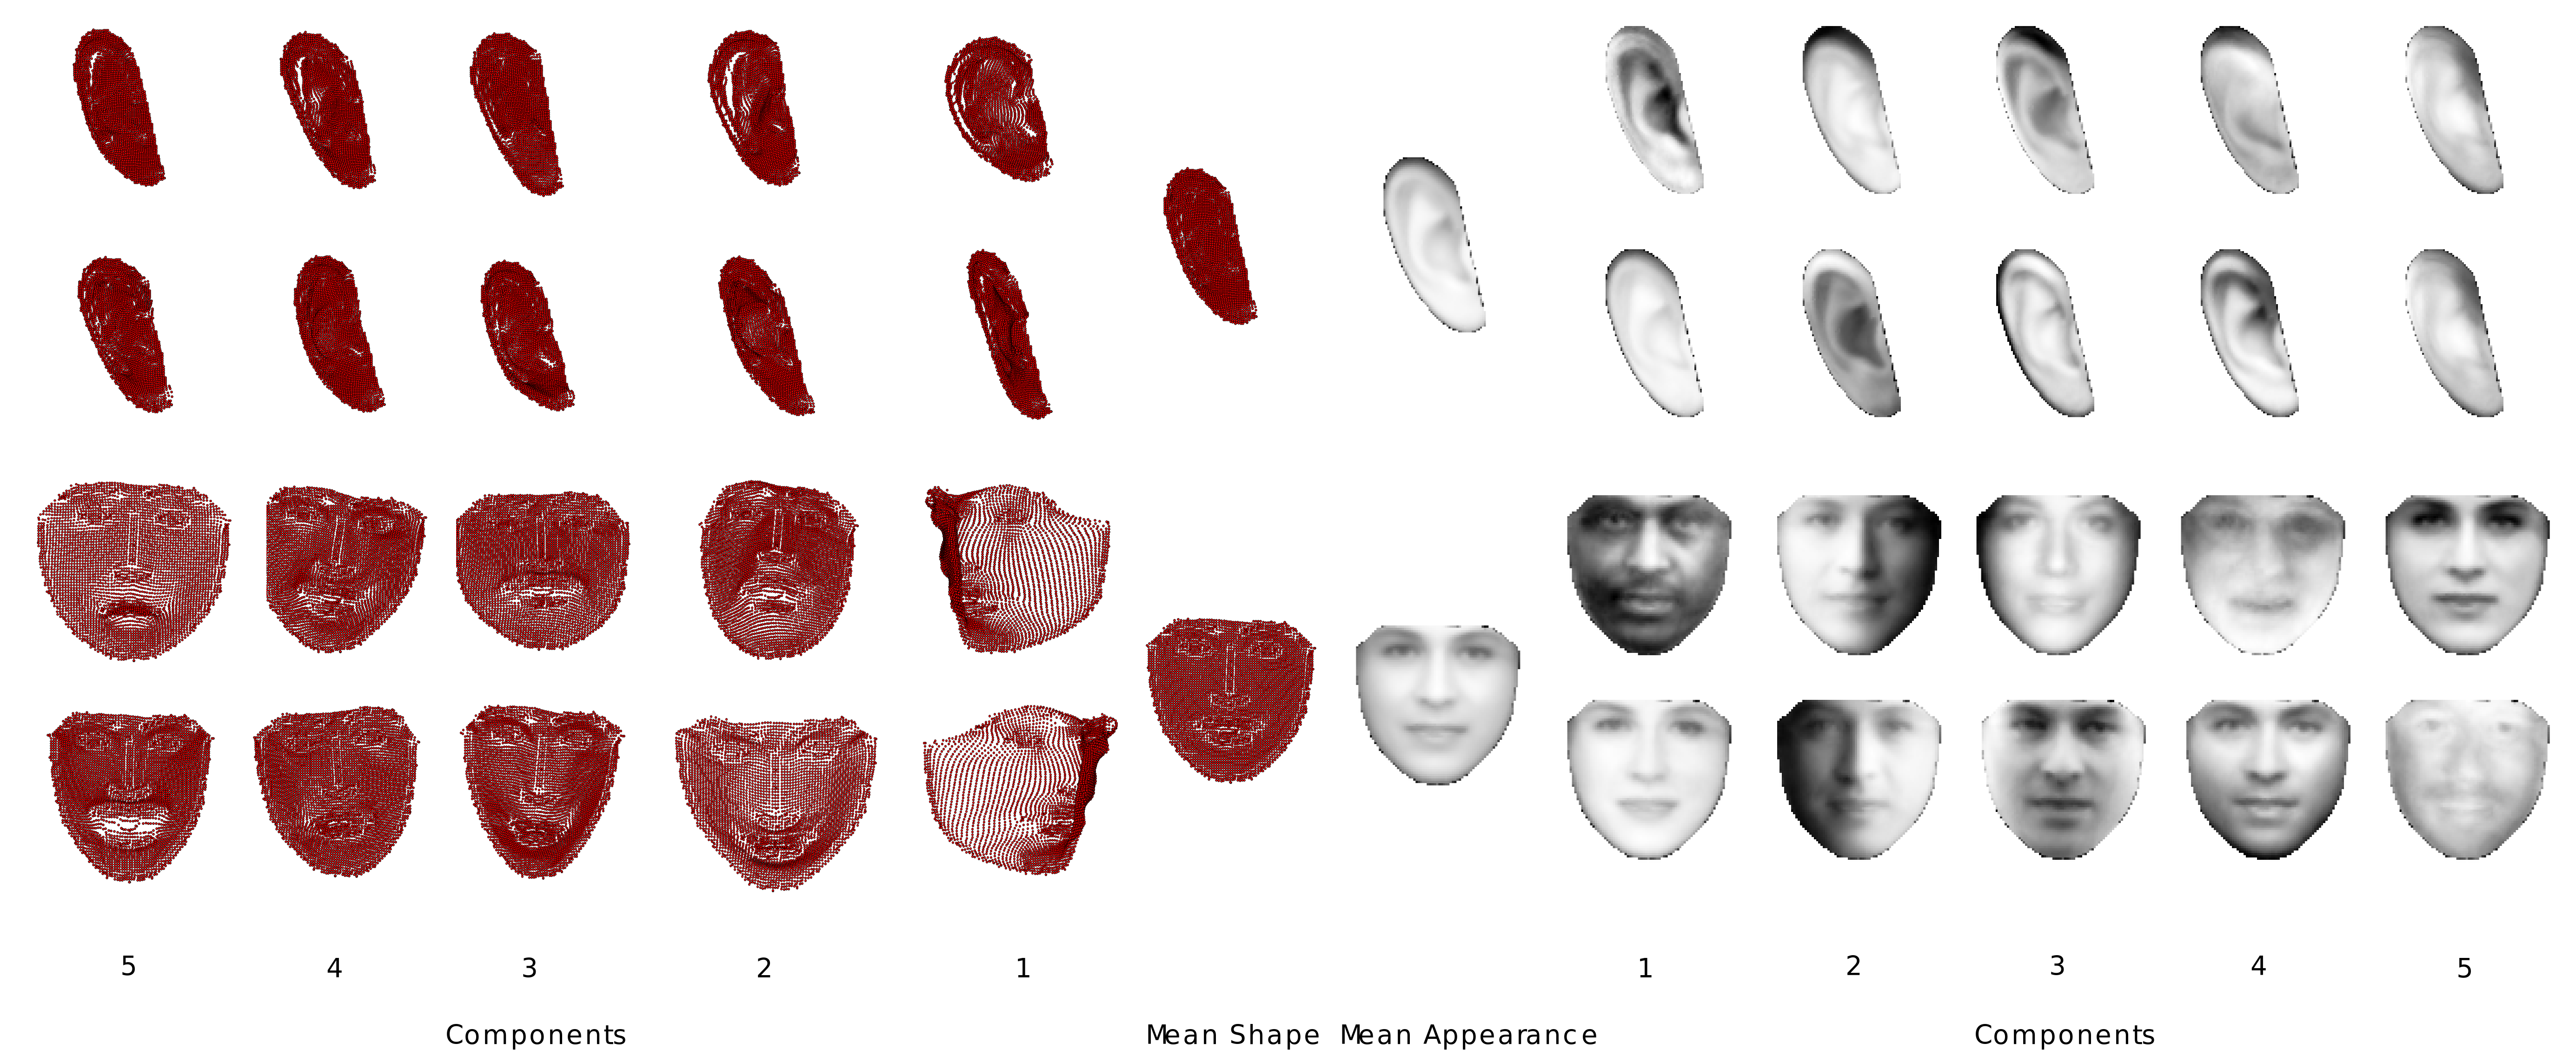
\includegraphics[width=\textwidth]{Suplementory_Meterial/Models/models}
\caption{Principal components of dAAMs built on ears (top) and faces (bottom). The mean (middle columns) as well as the first five principal components are visualised for both shape (left) and appearance (right). $\pm 3$ times the variance of the corresponding component is used in each case.}
\label{fig:pcamodel}
\end{figure*}


%%%%%%%%% Appendix
\section*{Introduction}
In this supplementary material, we provide additional algorithmic details for our shape flow estimation, as well as additional visualisations and evaluations for the dense and patch-based AAMs that were constructed using the proposed framework.


\appendix
\section{Implementation of Shape Flow Estimation}
\label{sec:cost_function}


As mentioned in the main submission (Section 3, Step 3), we propose to estimate the shape flow by minimising the following energy:
\vspace{-5pt}
\begin{align}
E_{sf} & =\alpha
\int_{\Omega}\sum_{n=1}^{N_t} \|\bm{d}(\bx+\bm{u}_n(x);n)-\bm{d}(x;0)\| \ud \bx \label{eq:costfunc}\\
    &+ \beta \int_{\Omega}\sum_{n=1}^{N_t}\|\bm{u}_n(\bx)-\sum_{i=1}^R\bm{q}_i(n)\bm{v}_i(\bx)\|^2 \ud \bx \label{eq:lowrank}\\
    &+
\int_\Omega  \sum_{i=1}^R \,\, \left \|    \nabla \bm{v}_i(\bx)    \right \|  \,\ud \bx \label{eq:TVterm}
\vspace{-5pt}
\end{align}
We minimise this energy jointly with respect to $\bm{u}_n(\bx)$ and $\bm{v}_i(\bx)$, which correspond to the
two sets of unknown shape flows.
We implement this minimisation based on the optimisation algorithm described in \cite{Garg:2013hu} and the relevant publicly available code \footnote{https://bitbucket.org/troussos/mfsf/downloads}.
However, we modify this algorithm so that, instead of initialising the coarse-to-fine and warping iterations with a zero flow, we use Thin Plate Splines (TPS) \cite{Bookstein1989} interpolation of the initial correspondence vectors described in Section 3, Step 2 of the main submission.
This yields a significantly better initial location of the highly-nonconvex objective function and improves the computational efficiency, since much less coarse-to-fine pyramids are needed.

Note that in every coarse-to-fine and warping iteration, we use an initialisation that comes from the previous iteration. We approximate the data term \eqref{eq:costfunc} by linearising the SVS images $\bm{d}(\bx;n)$ around the initialisation. After that, the energy becomes convex and we optimise it by employing alternating optimisation with respect to $\bm{v}_i(\bx)$ and $\bm{u}_n(\bx)$. The minimisation with respect to $\bm{v}_i(\bx)$ is decoupled for every coefficient $i$ and corresponds to Rudin-Osher-Fatemi Total Variation denoising~\cite{rudin92}, which we solve efficiently by applying the first order primal-dual algorithm of~\cite{Chambolle:Pock:JMIV2011}. The minimisation with respect to $\bm{u}_n(x)$ is decoupled for every pixel $\bx$ and every shape index $i$. This minimisation is also implemented by applying the efficient primal-dual algorithm of~\cite{Chambolle:Pock:JMIV2011}.

\section{Dense Active Appearance Models}
\label{sec:daam}

In this section, we report additional qualitative and quantitative evaluations for the Dense Active Appearance Models (dAAMs) of faces and ears that were constructed using the proposed framework.



\subsection{Principal Components and Compactness}



Figure~\ref{fig:pcamodel} visualises the first five shape and appearance principal components of ear and face dAAMs. We observe that in both ear and face cases, the variation of both shape and appearance captured by the model seem plausible.


Figure~\ref{fig:compact} pliots the variance ration of the face dAAM, which provides an indication of the compactness of the model. The compactness is compared with the one of a standard sparse AAM built on the same data. Note that these are the two shape models that are compared in Figure 9-left of the main paper. We observe that our dAAM is significantly more compact than the sparse AAM, since for any given number of components, it manages to explain a larger portion of the corresponding total variance of the training set. 


\begin{figure}[!t]
    \centering
    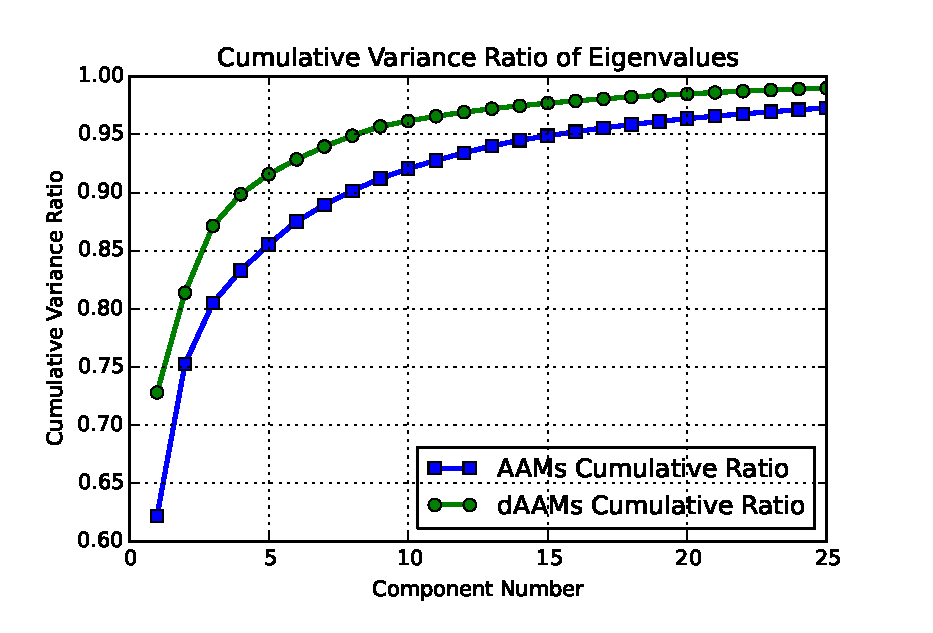
\includegraphics[width=\columnwidth]{Suplementory_Meterial/Model_Analysis/cumu_var_ratio}
    \caption{Compactness plots of dAAM (green) and sparse AAM (blue) models for faces. Portion of the corresponding total variance explained as a function of the number of retained principal components.}
    \label{fig:compact}
\end{figure}

\subsection{Dense Shape Reconstruction Ability}

\begin{figure}[!t]
    \centering
    % \vspace*{-0.1in}
    \begin{subfigure}[b]{\columnwidth}
            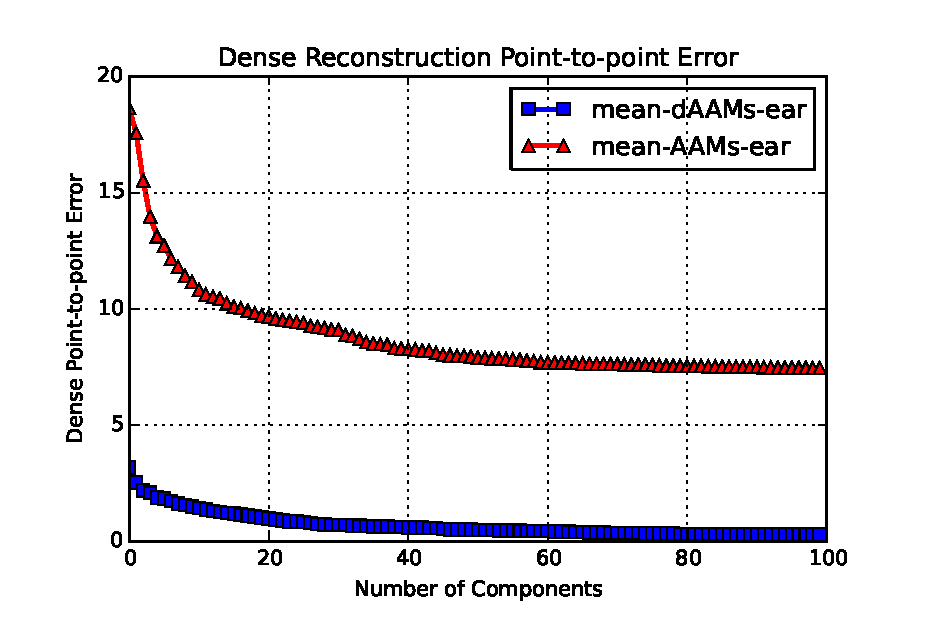
\includegraphics[width=\textwidth,trim={0 0 0 25pt},clip]{Suplementory_Meterial/Model_Analysis/sr_ear}
        %\caption{dAAMs dense shape reconstruction}
    \end{subfigure}
    \\
    \begin{subfigure}[b]{\columnwidth}
            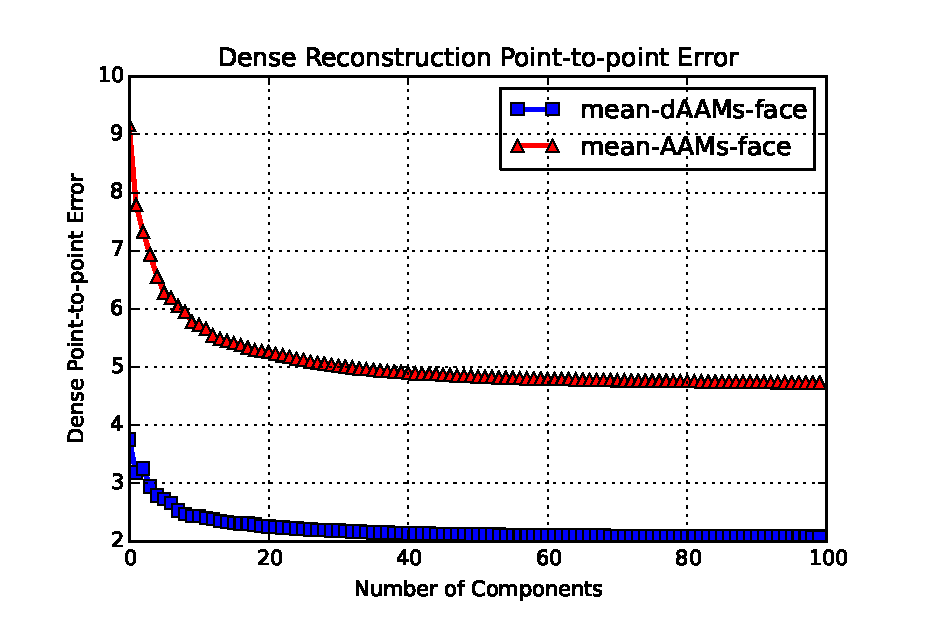
\includegraphics[width=\textwidth,trim={0 0 0 25pt},clip]{Suplementory_Meterial/Model_Analysis/sr_face}
        %\caption{AAMs dense shape reconstruction}
    \end{subfigure}
    \caption{Dense shape reconstruction errors for ears (top) and faces (bottom), using AAMs (red) and dAAMs (blue). The average normalized dense point-to-point distance error is plotted as a function of the number of principal components of the model.}
    \label{fig:rc_face}
\end{figure}

Figure \ref{fig:rc_face} evaluates the dense shape reconstruction ability of the proposed dAAMs and compares it with that of standard sparse AAMs. Specifically, we use shapes with dense ground-truth annotations and reconstruct them with both AAMs and dAAMs, by projecting on the corresponding model subspace. In the case of AAMs, which only contain a sparse shape model, we densify it using a piecewise affine transformation, which is typically for texture warping of these models. We observe that dAAMs significantly outperform classic AAMs, in terms of dense shape reconstruction accuracy.



\begin{figure*}[!t]
    \newcommand{\ofh}{0.24\columnwidth}
    \centering
    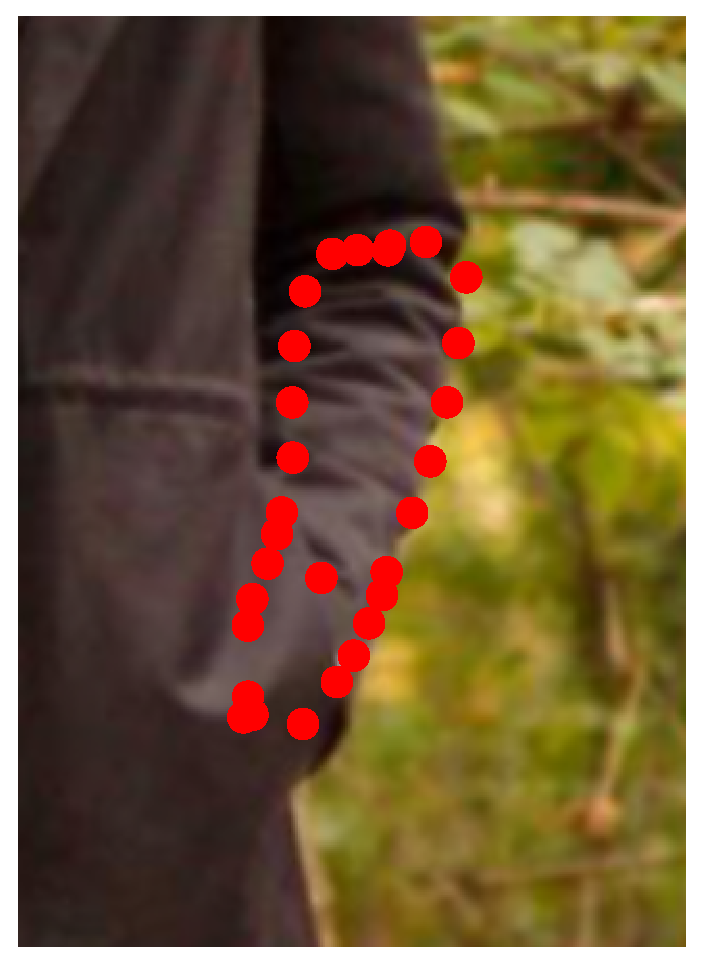
\includegraphics[height=\ofh]{Suplementory_Meterial/ExFit/0001.eps}
    \hfill
    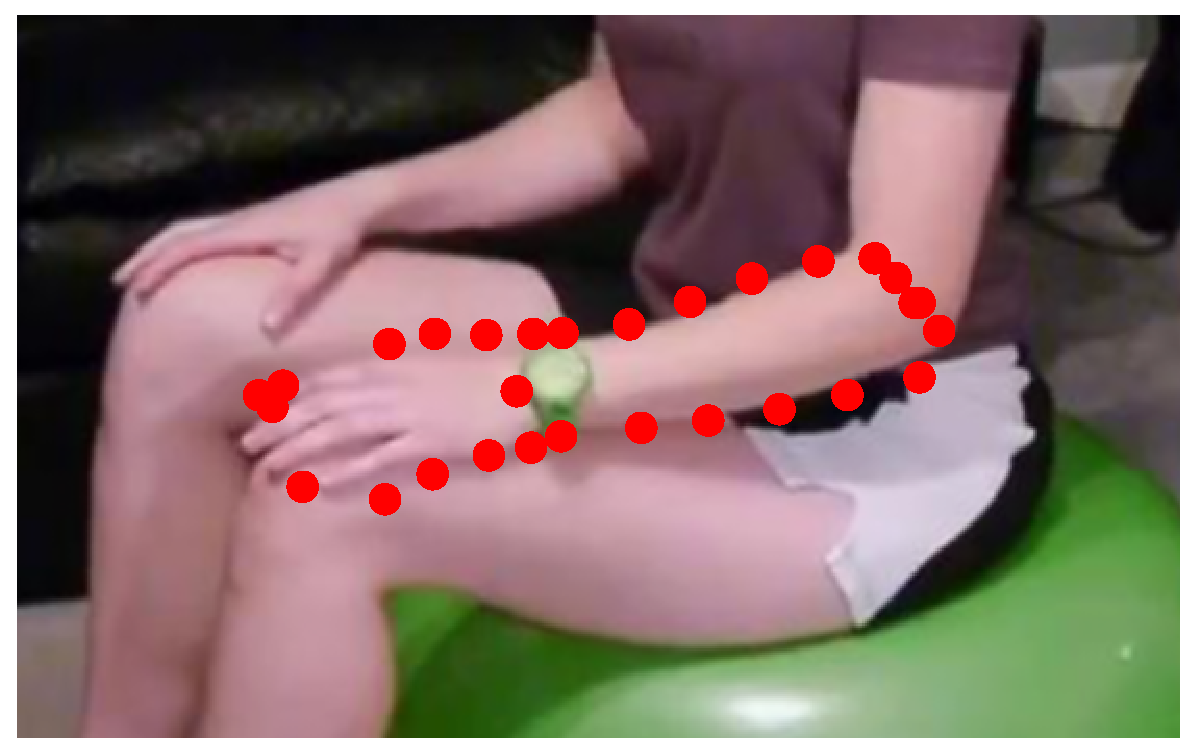
\includegraphics[height=\ofh]{Suplementory_Meterial/ExFit/0002.eps}
    \hfill
    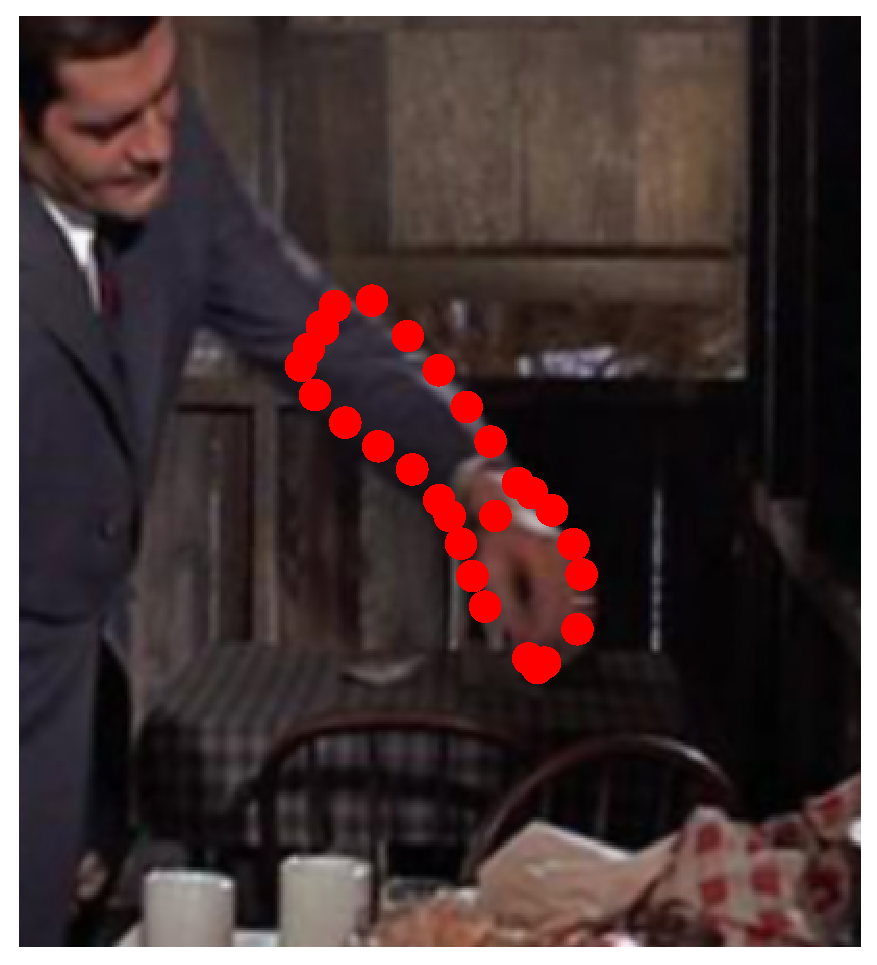
\includegraphics[height=\ofh]{Suplementory_Meterial/ExFit/0003.eps}
    \hfill
    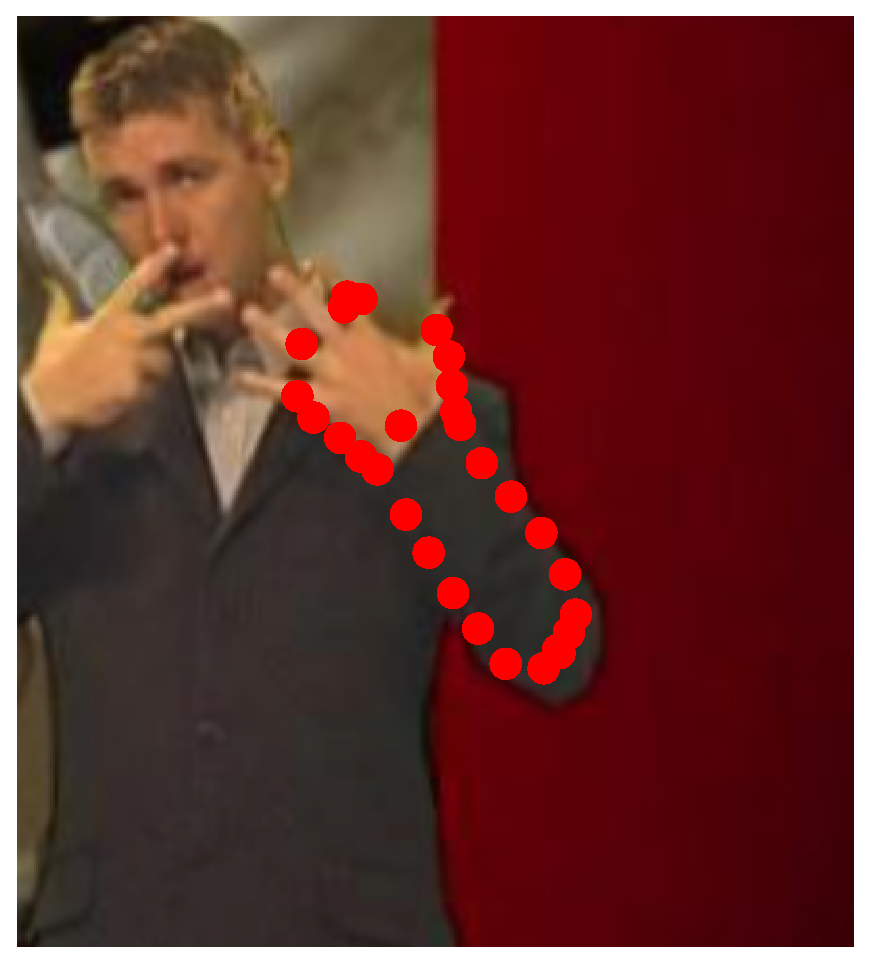
\includegraphics[height=\ofh]{Suplementory_Meterial/ExFit/0004.eps}
    \hfill
    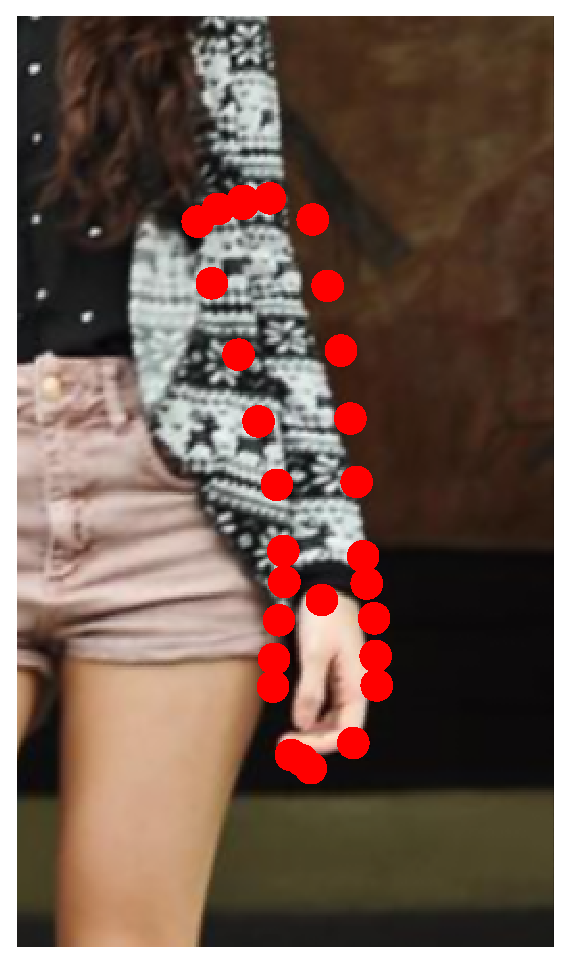
\includegraphics[height=\ofh]{Suplementory_Meterial/ExFit/0005.eps}
    \hfill
    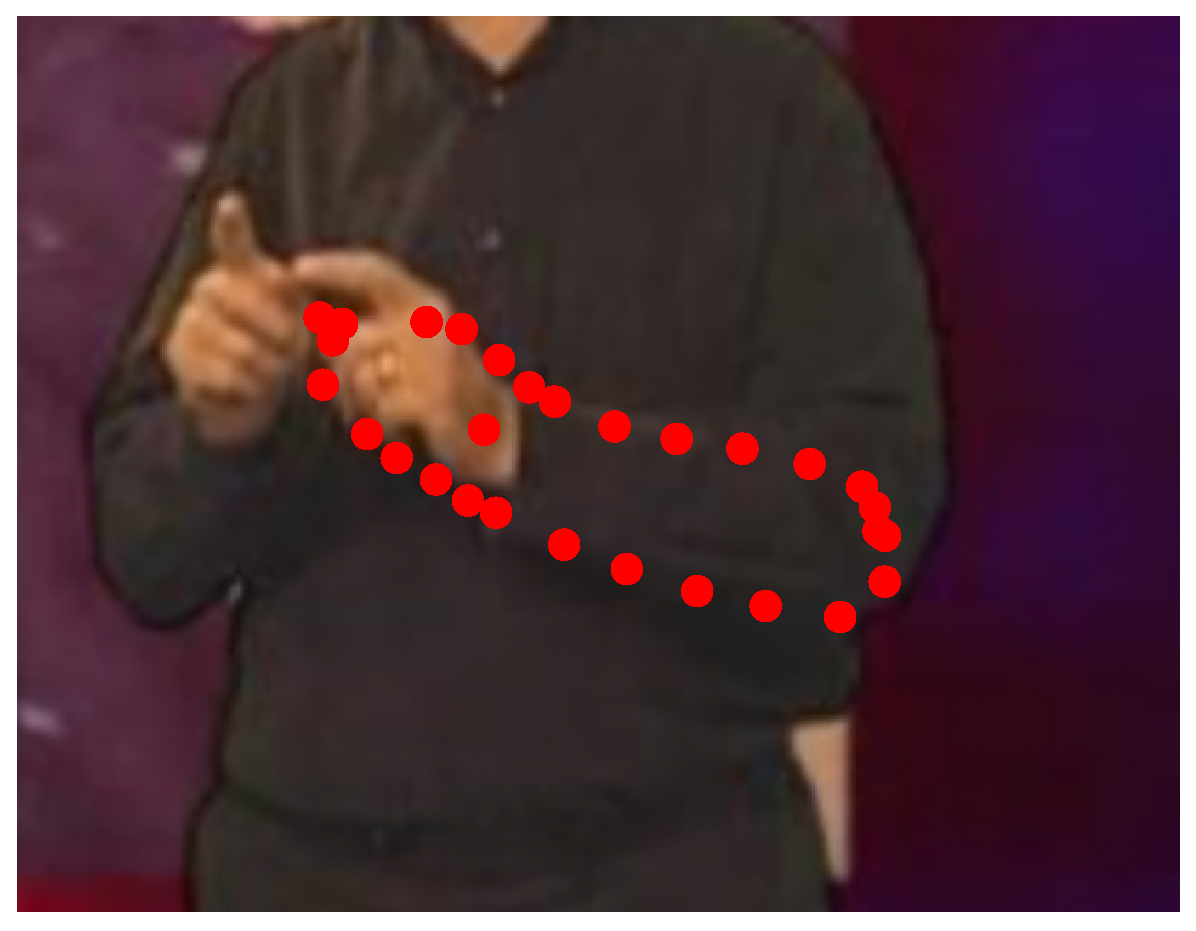
\includegraphics[height=\ofh]{Suplementory_Meterial/ExFit/0006.eps}
    \hfill
    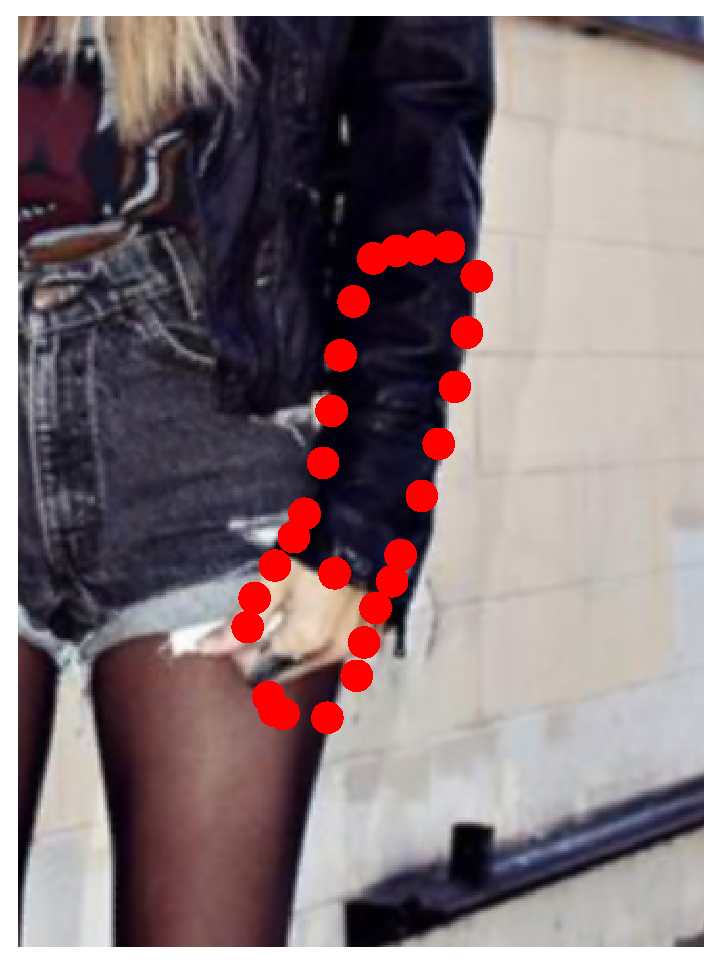
\includegraphics[height=\ofh]{Suplementory_Meterial/ExFit/0007.eps}
    \hfill
    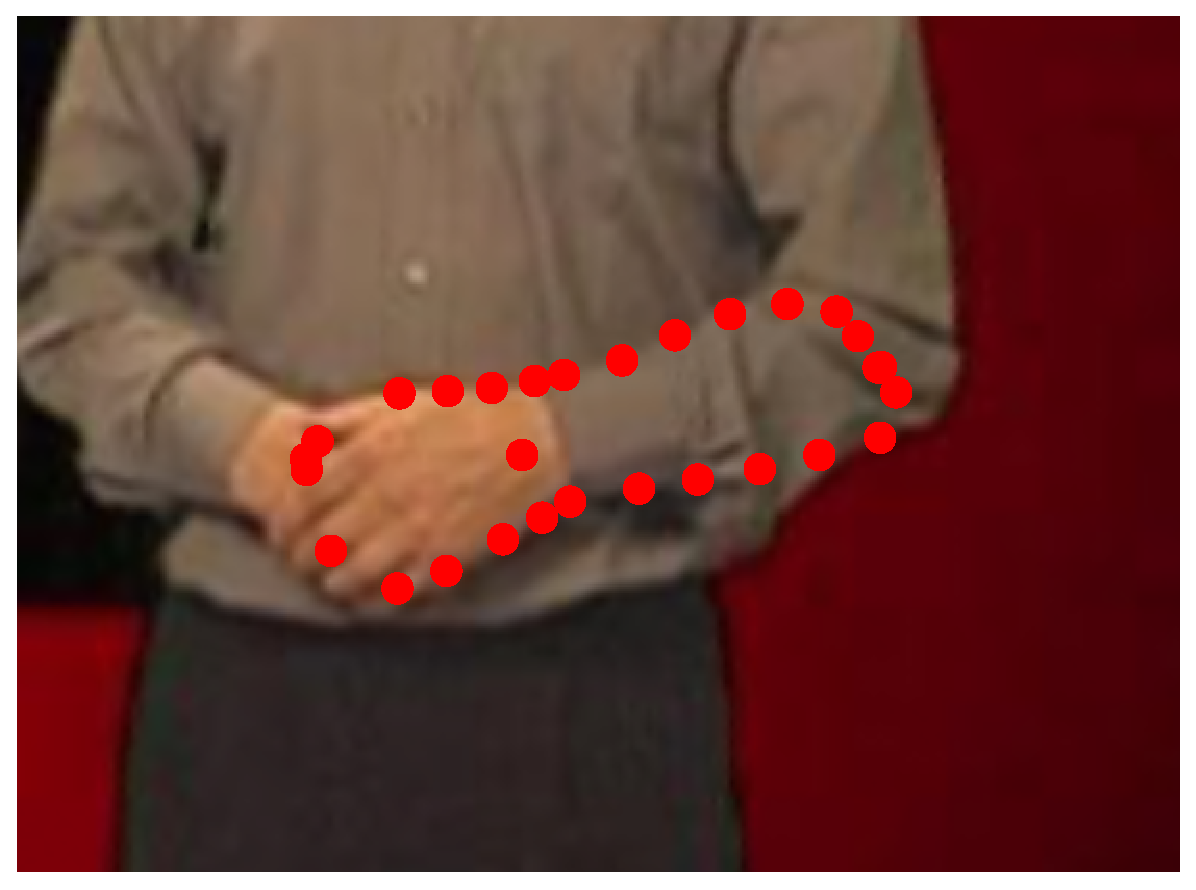
\includegraphics[height=\ofh]{Suplementory_Meterial/ExFit/0008.eps}
    \hfill
    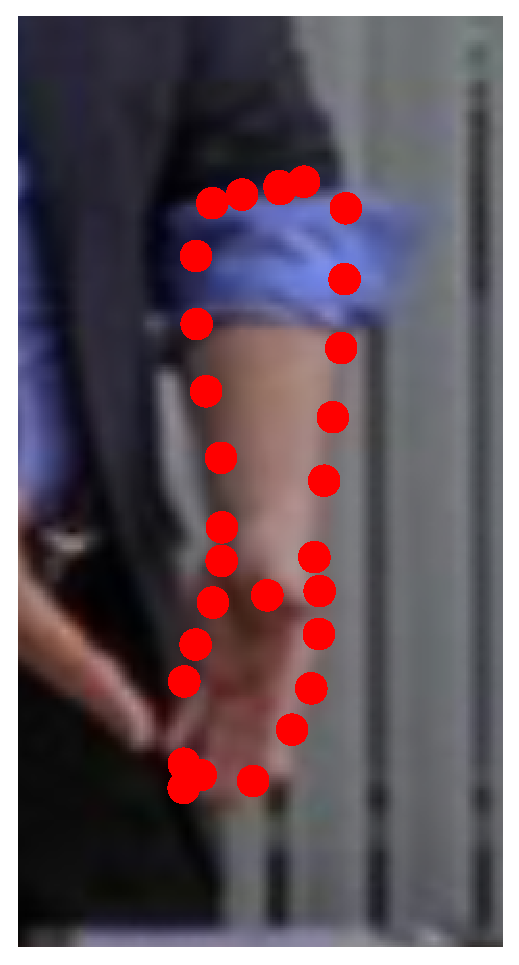
\includegraphics[height=\ofh]{Suplementory_Meterial/ExFit/0009.eps}
    \hfill
    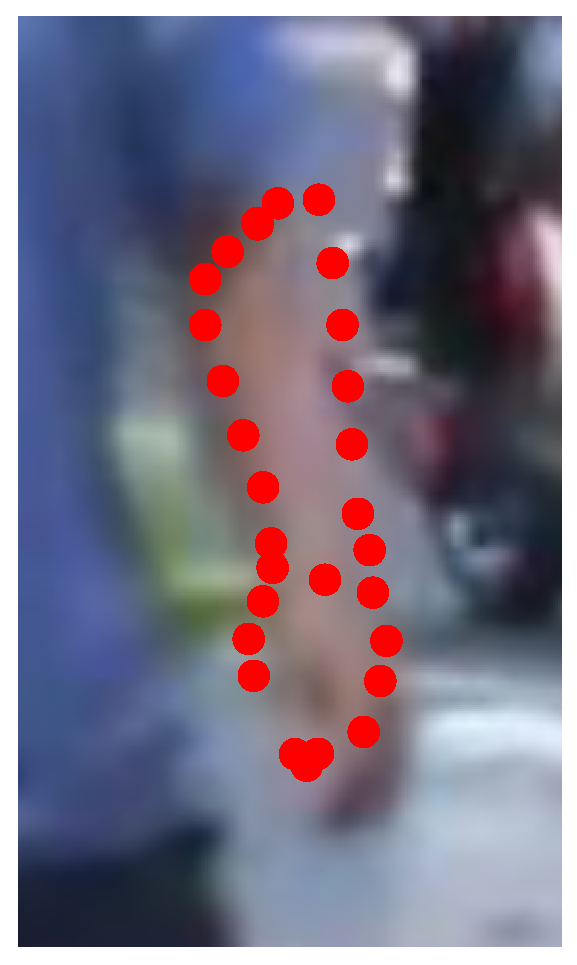
\includegraphics[height=\ofh]{Suplementory_Meterial/ExFit/0010.eps}
    \hfill
    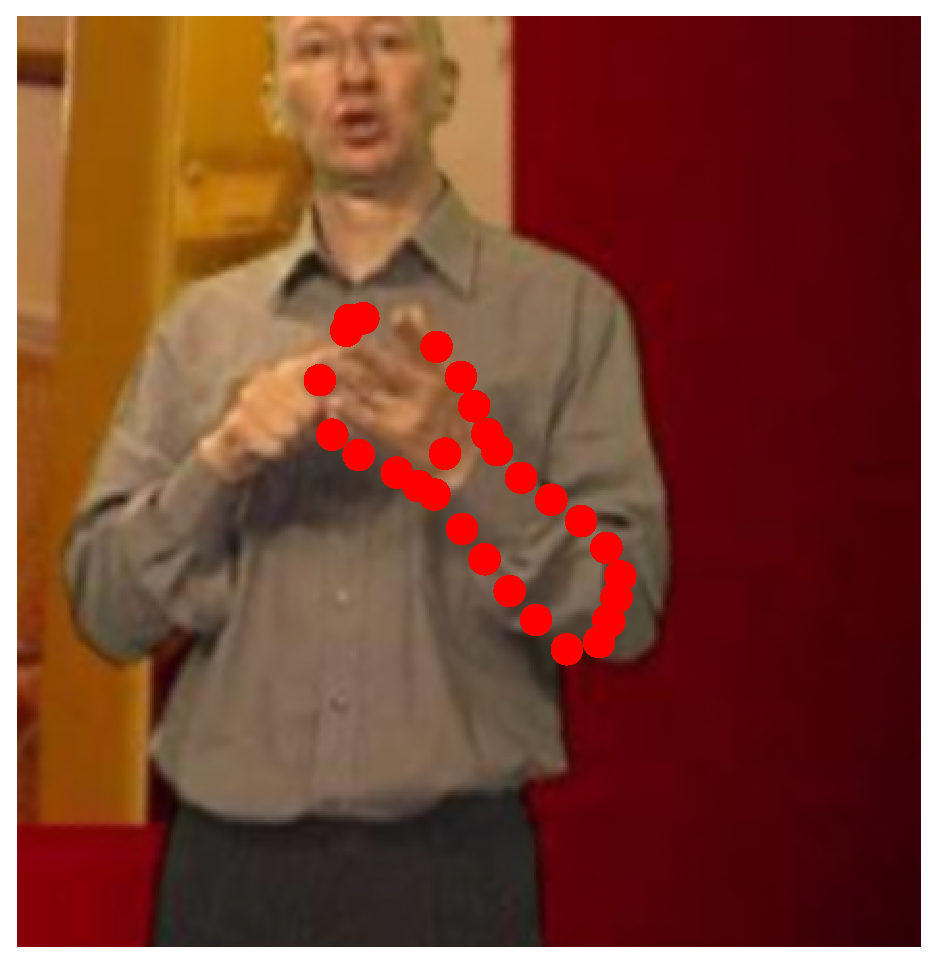
\includegraphics[height=\ofh]{Suplementory_Meterial/ExFit/0011.eps}
    \hfill
    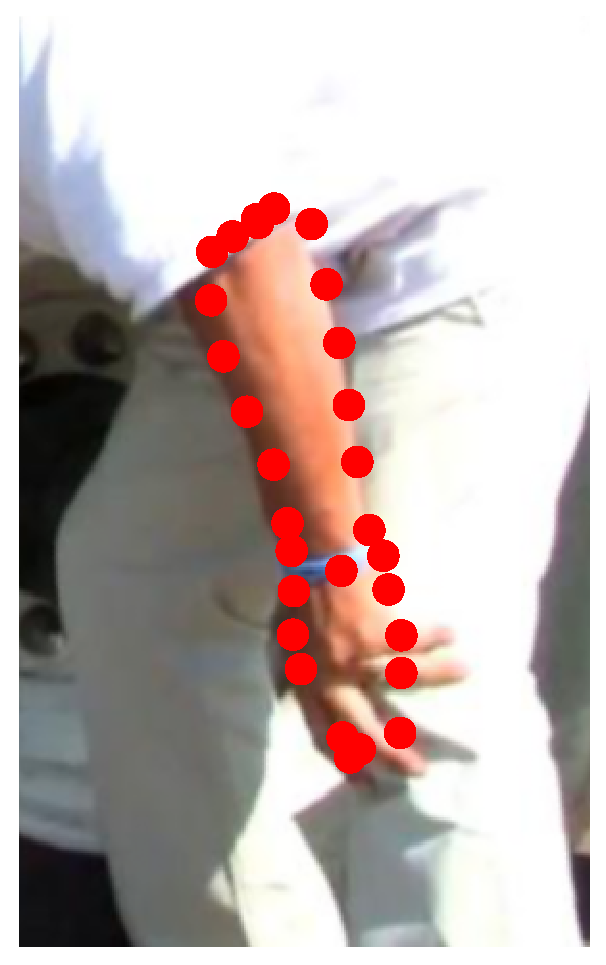
\includegraphics[height=\ofh]{Suplementory_Meterial/ExFit/0012.eps}
    \hfill
    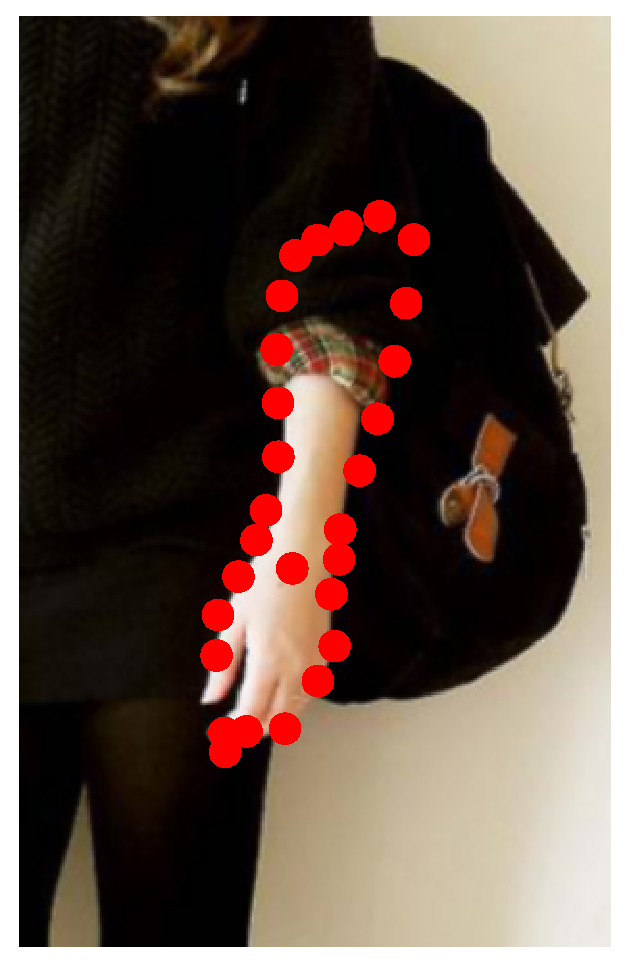
\includegraphics[height=\ofh]{Suplementory_Meterial/ExFit/0013.eps}
    \hfill
    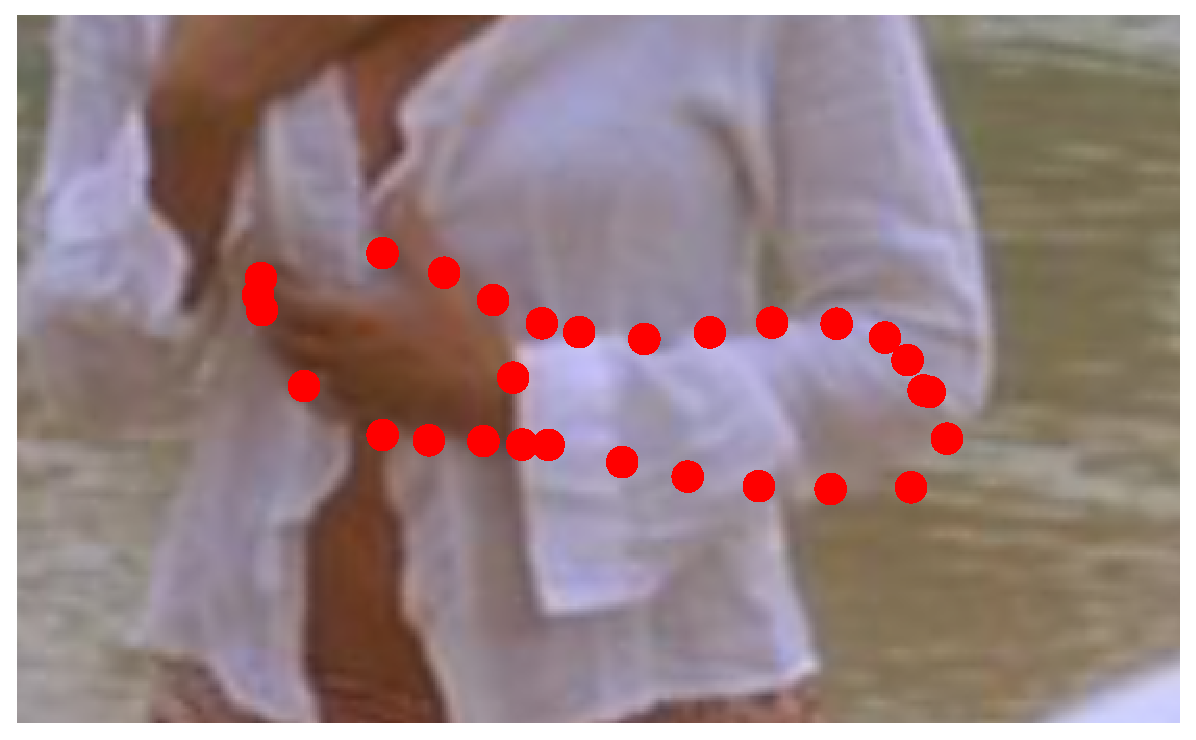
\includegraphics[height=\ofh]{Suplementory_Meterial/ExFit/0014.eps}
    \hfill
    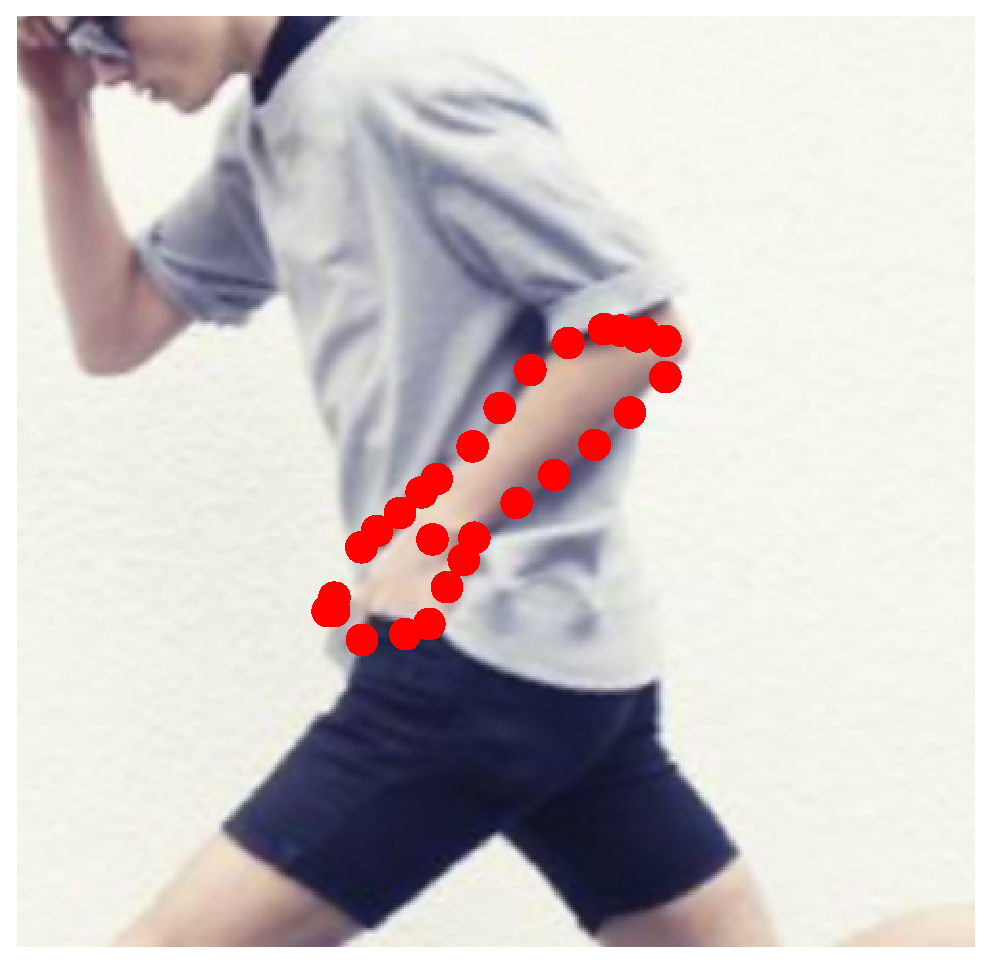
\includegraphics[height=\ofh]{Suplementory_Meterial/ExFit/0015.eps}
    \hfill
    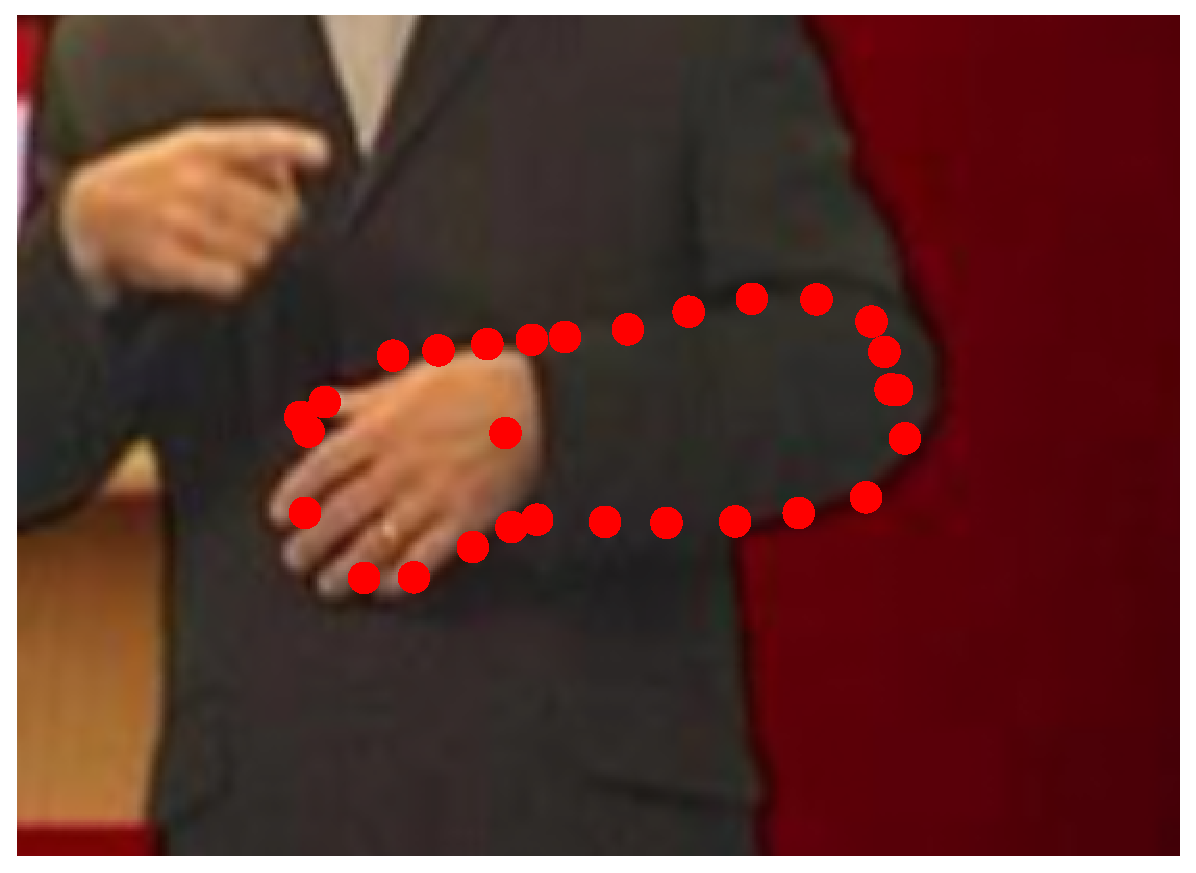
\includegraphics[height=\ofh]{Suplementory_Meterial/ExFit/0017.eps}
    \hfill
    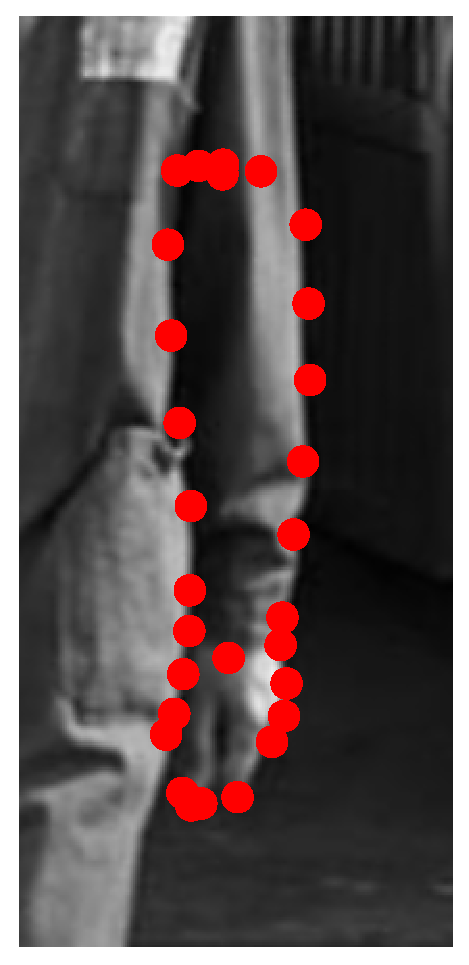
\includegraphics[height=\ofh]{Suplementory_Meterial/ExFit/0018.eps}
    \hfill
    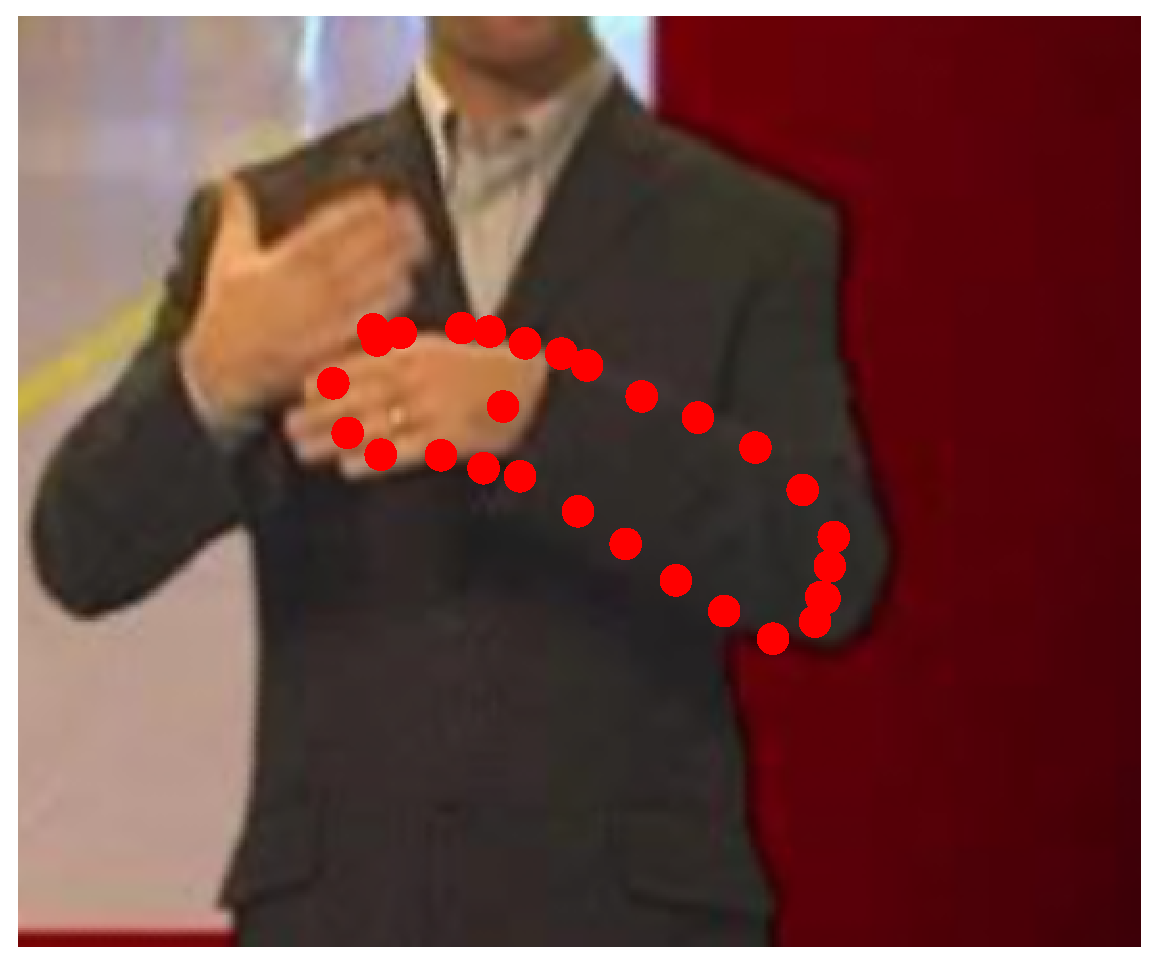
\includegraphics[height=\ofh]{Suplementory_Meterial/ExFit/0019.eps}
    \hfill
    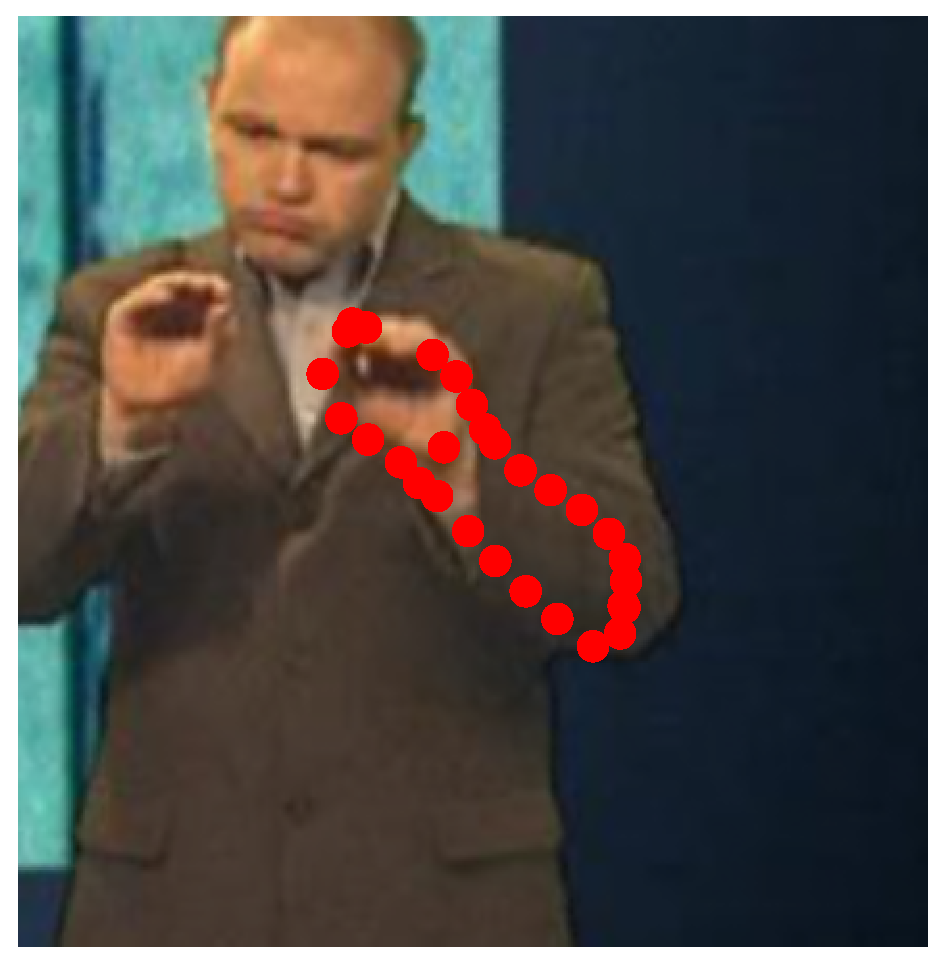
\includegraphics[height=\ofh]{Suplementory_Meterial/ExFit/0020.eps}
    \hfill
    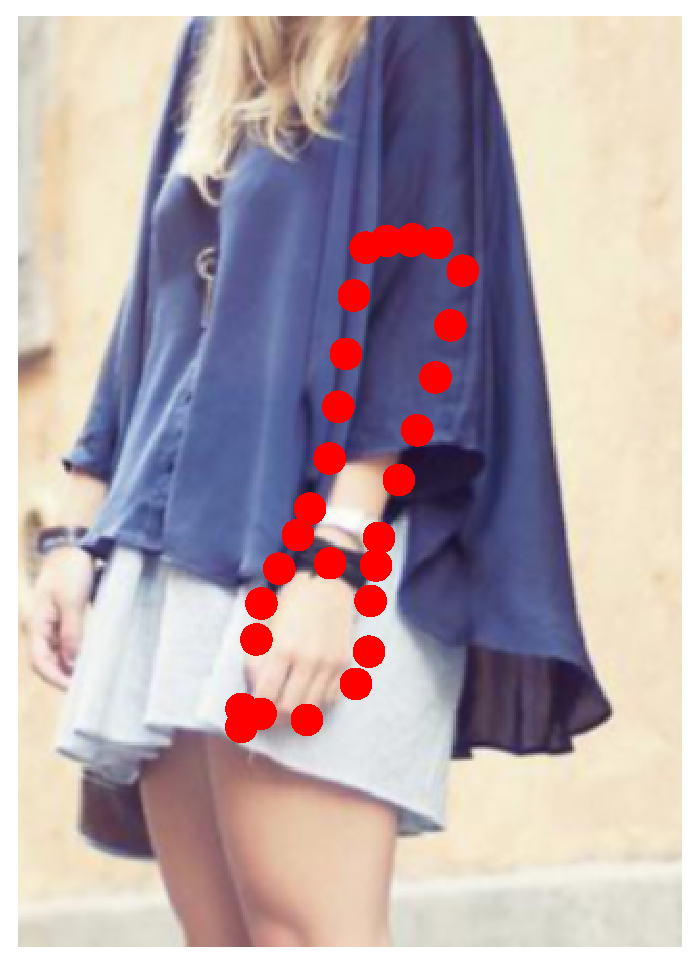
\includegraphics[height=\ofh]{Suplementory_Meterial/ExFit/0021.eps}
    \hfill
    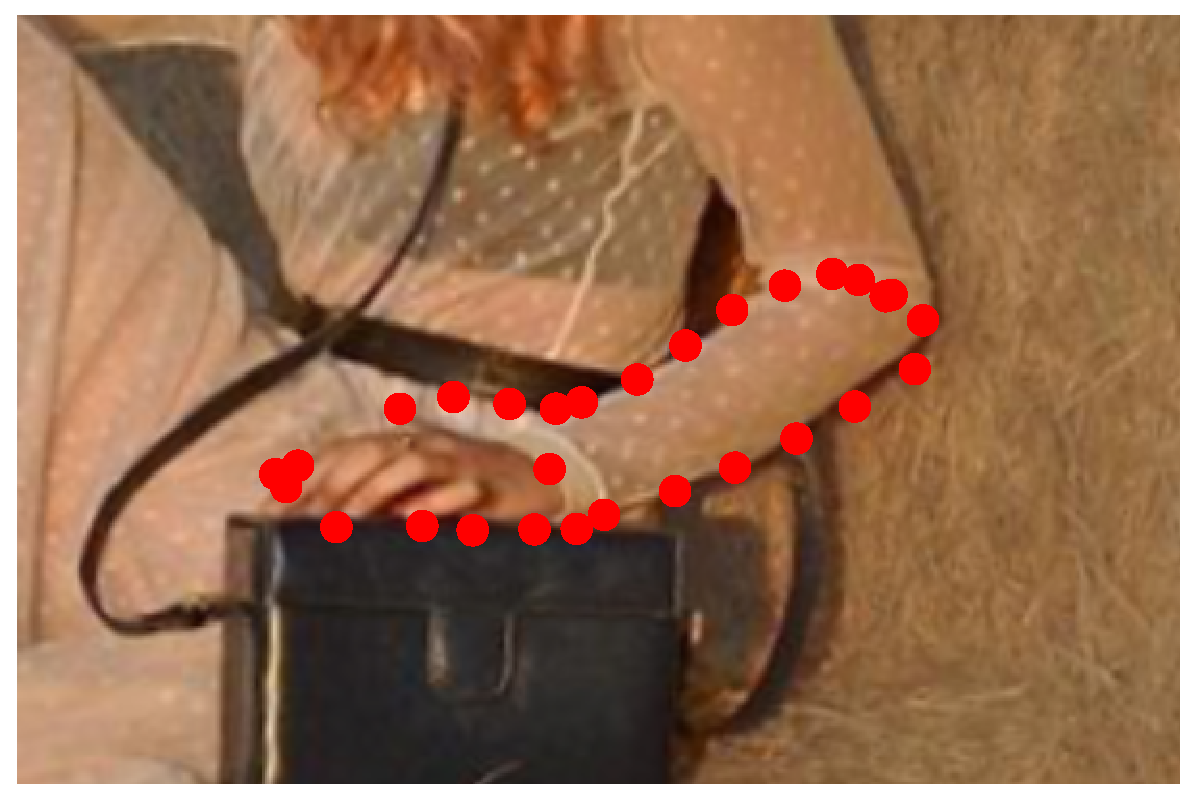
\includegraphics[height=\ofh]{Suplementory_Meterial/ExFit/0022.eps}
    \hfill
    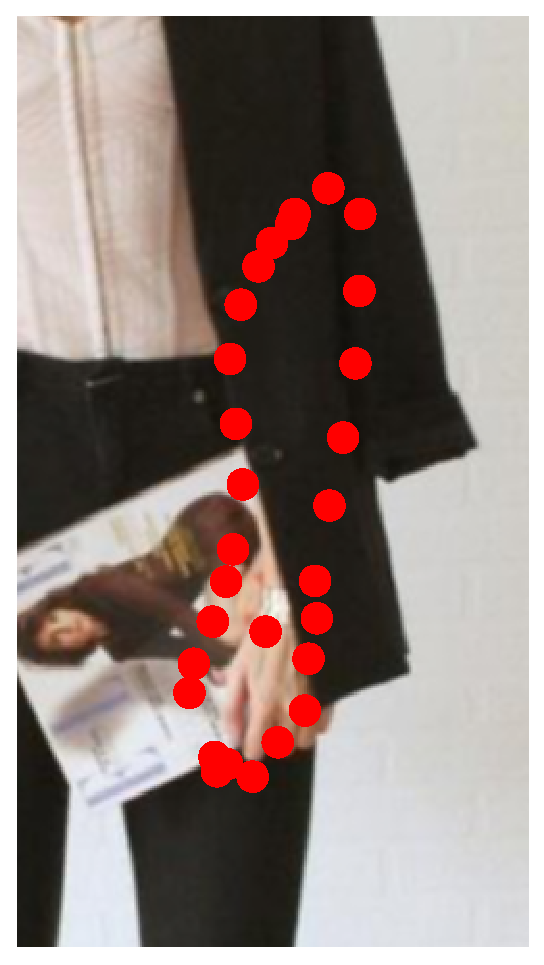
\includegraphics[height=\ofh]{Suplementory_Meterial/ExFit/0023.eps}
    \hfill
    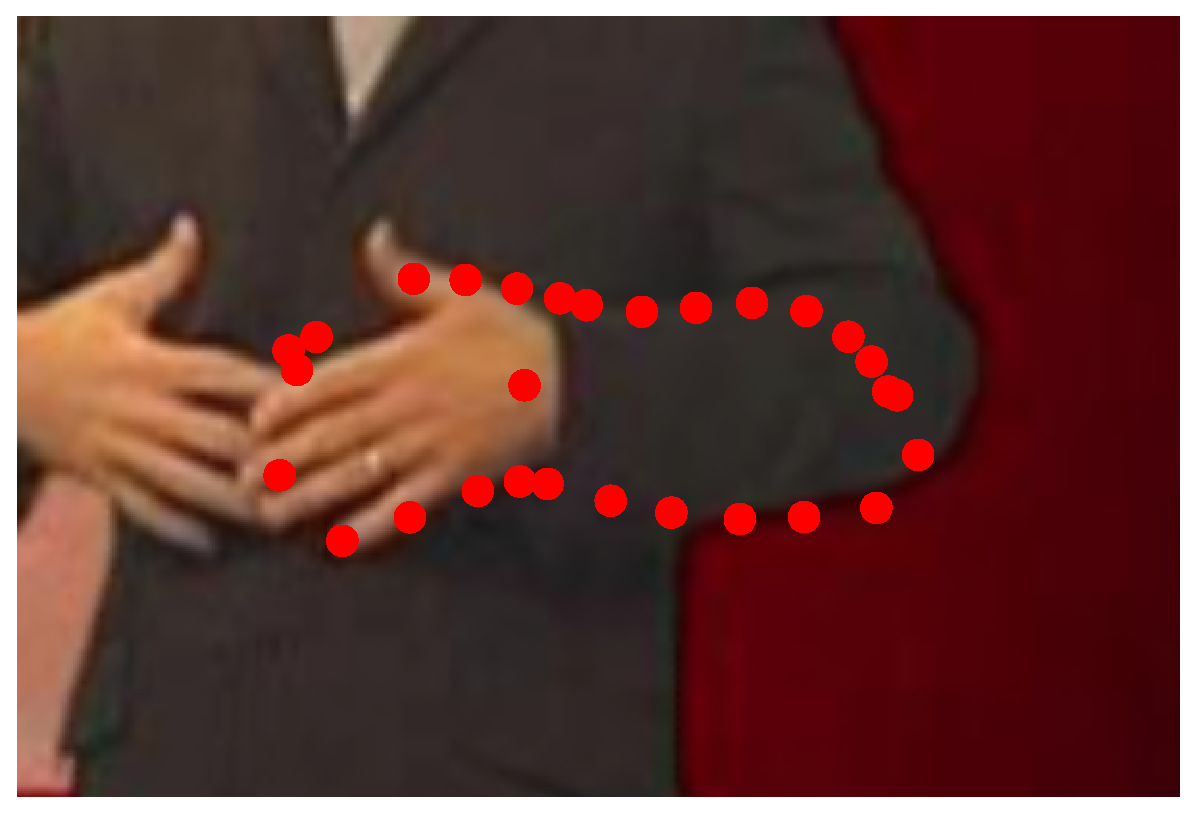
\includegraphics[height=\ofh]{Suplementory_Meterial/ExFit/0024.eps}
    \hfill
    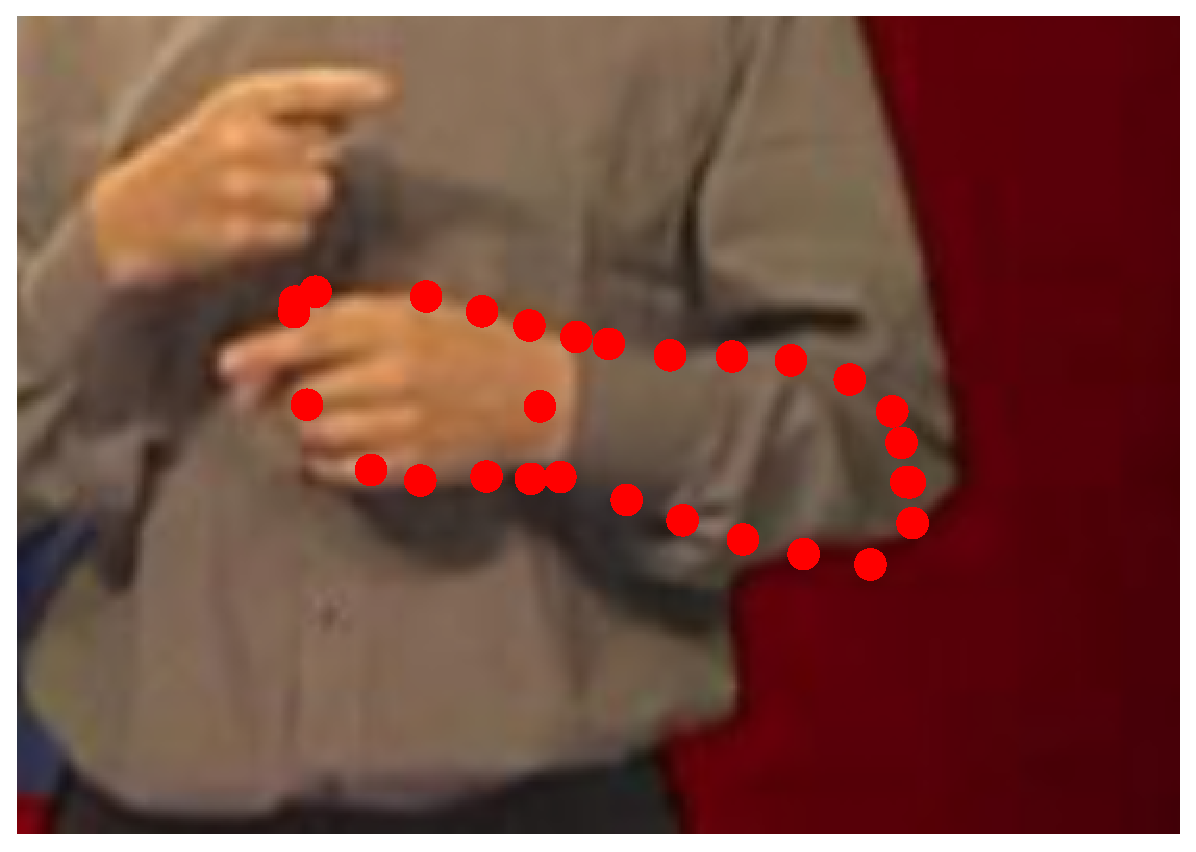
\includegraphics[height=\ofh]{Suplementory_Meterial/ExFit/0025.eps}
    \hfill
    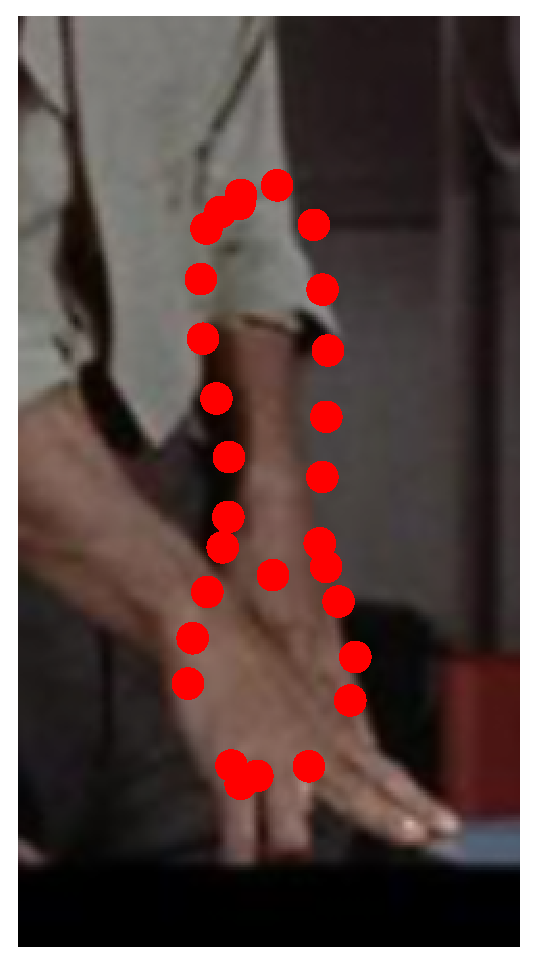
\includegraphics[height=\ofh]{Suplementory_Meterial/ExFit/0026.eps}
    \hfill
    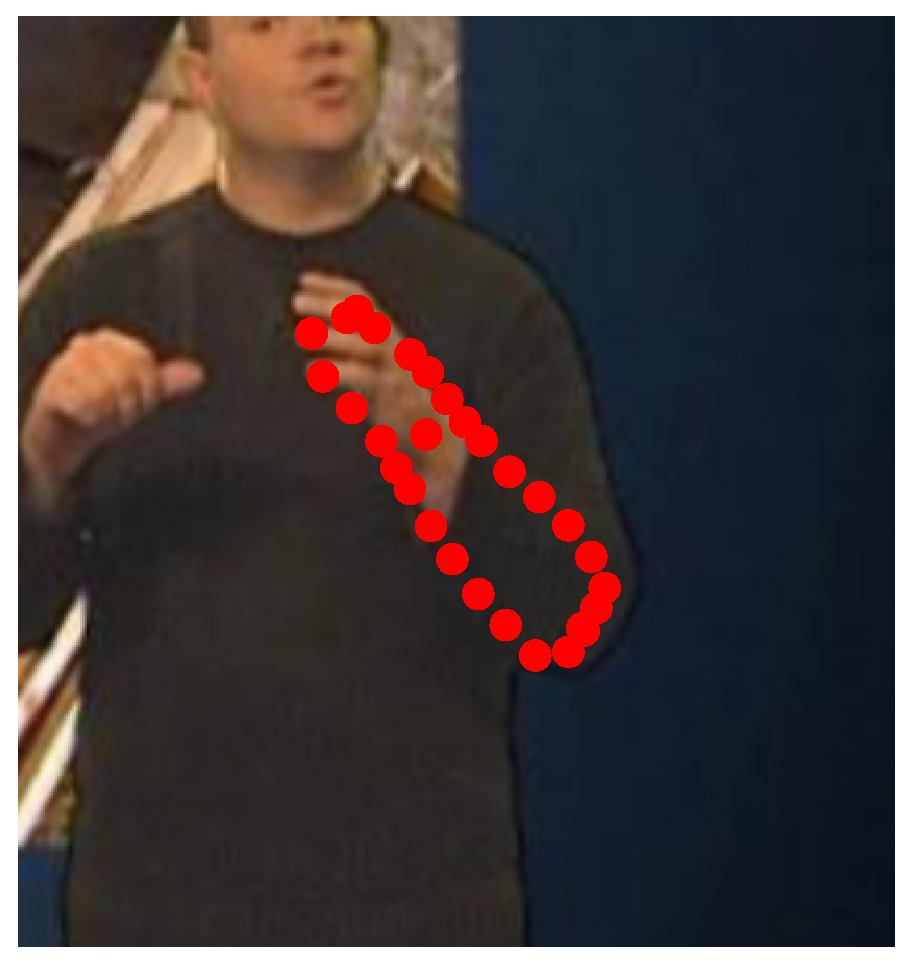
\includegraphics[height=\ofh]{Suplementory_Meterial/ExFit/0027.eps}
    \hfill
    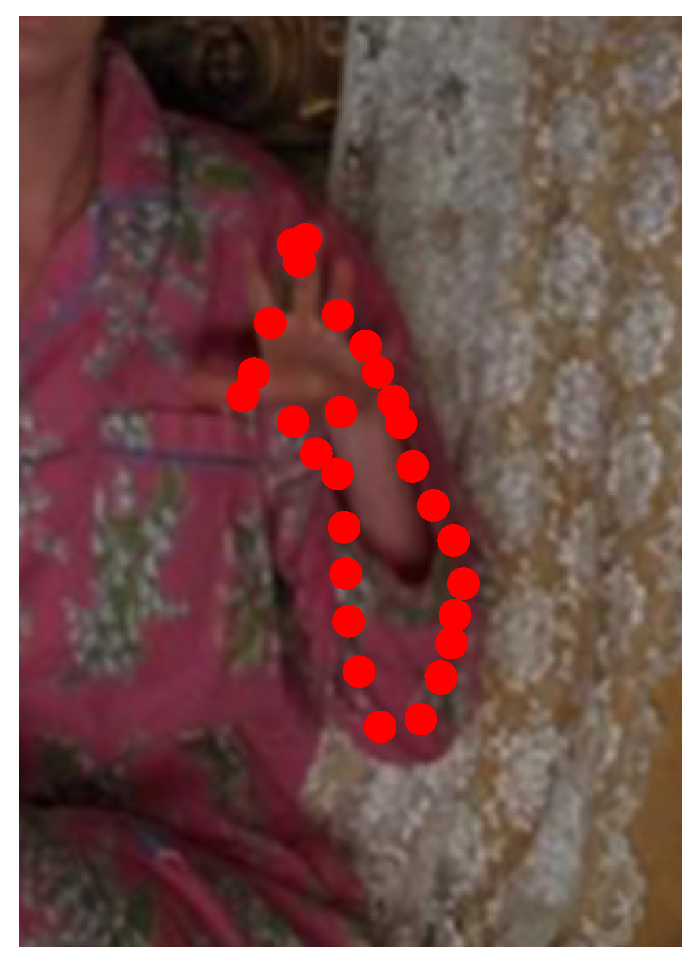
\includegraphics[height=\ofh]{Suplementory_Meterial/ExFit/0028.eps}
    \hfill
    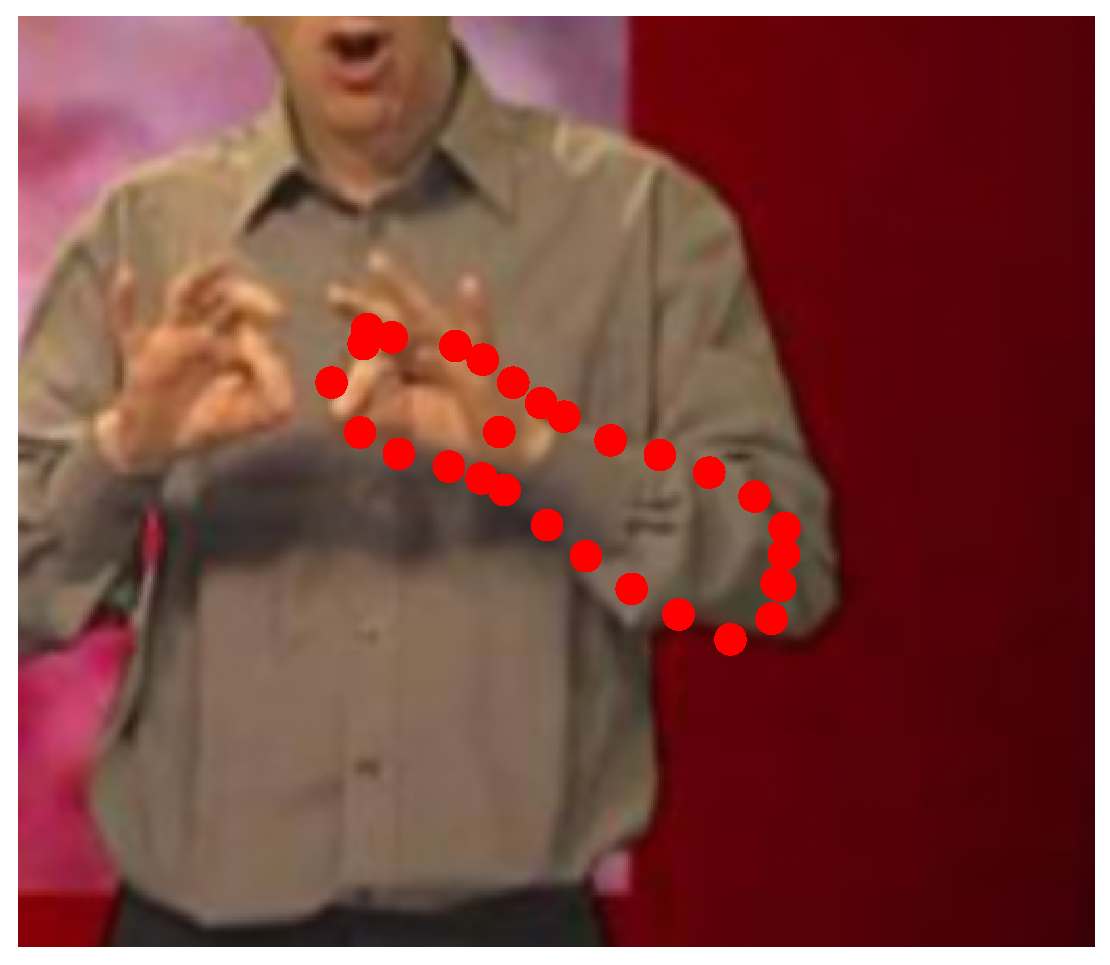
\includegraphics[height=\ofh]{Suplementory_Meterial/ExFit/0029.eps}
    \hfill
    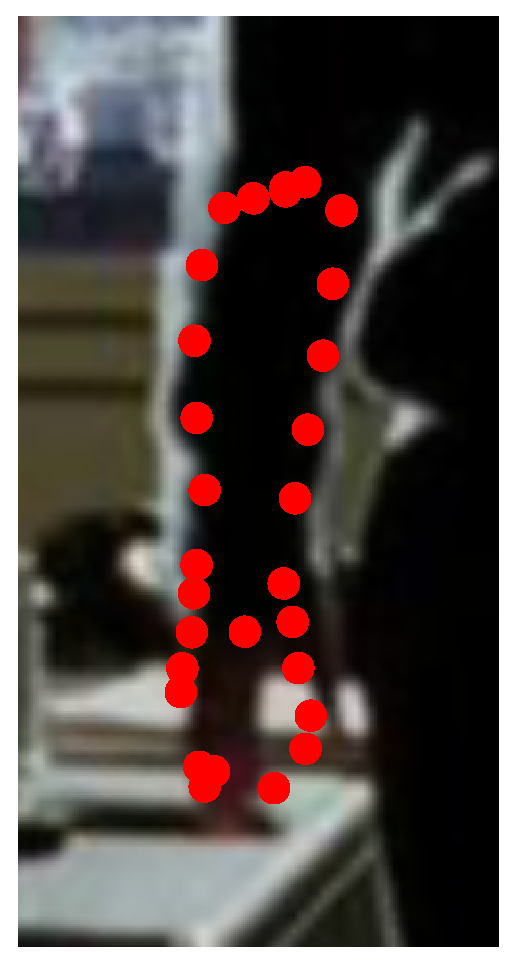
\includegraphics[height=\ofh]{Suplementory_Meterial/ExFit/0030.eps}
    \hfill
    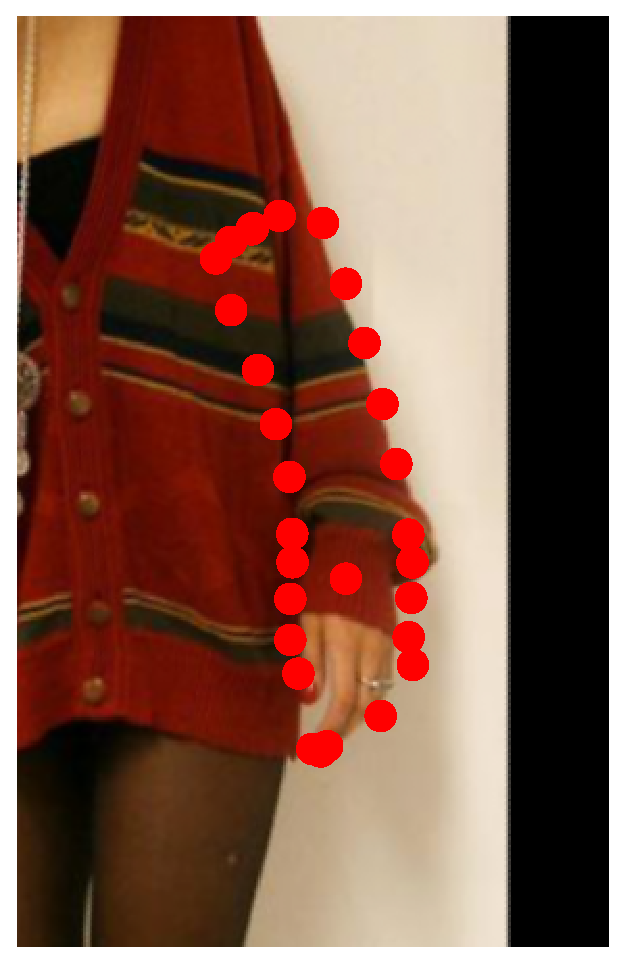
\includegraphics[height=\ofh]{Suplementory_Meterial/ExFit/0031.eps}
    \hfill
    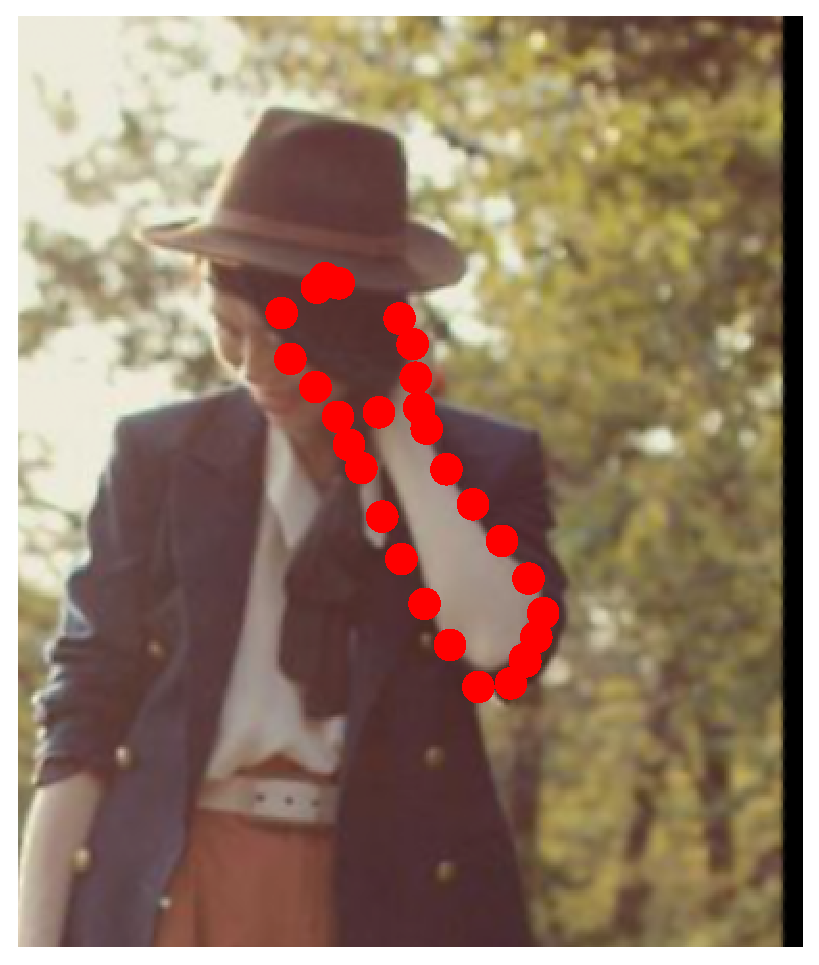
\includegraphics[height=\ofh]{Suplementory_Meterial/ExFit/0032.eps}
    \hfill
    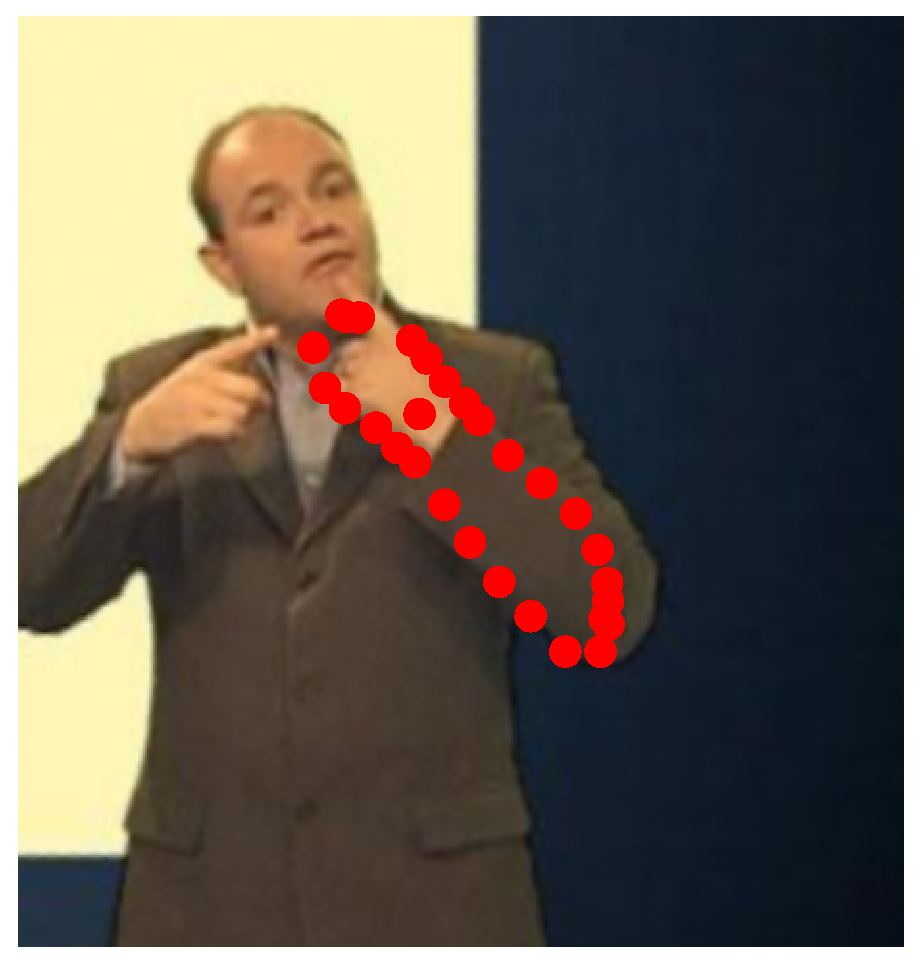
\includegraphics[height=\ofh]{Suplementory_Meterial/ExFit/0033.eps}
    \hfill
    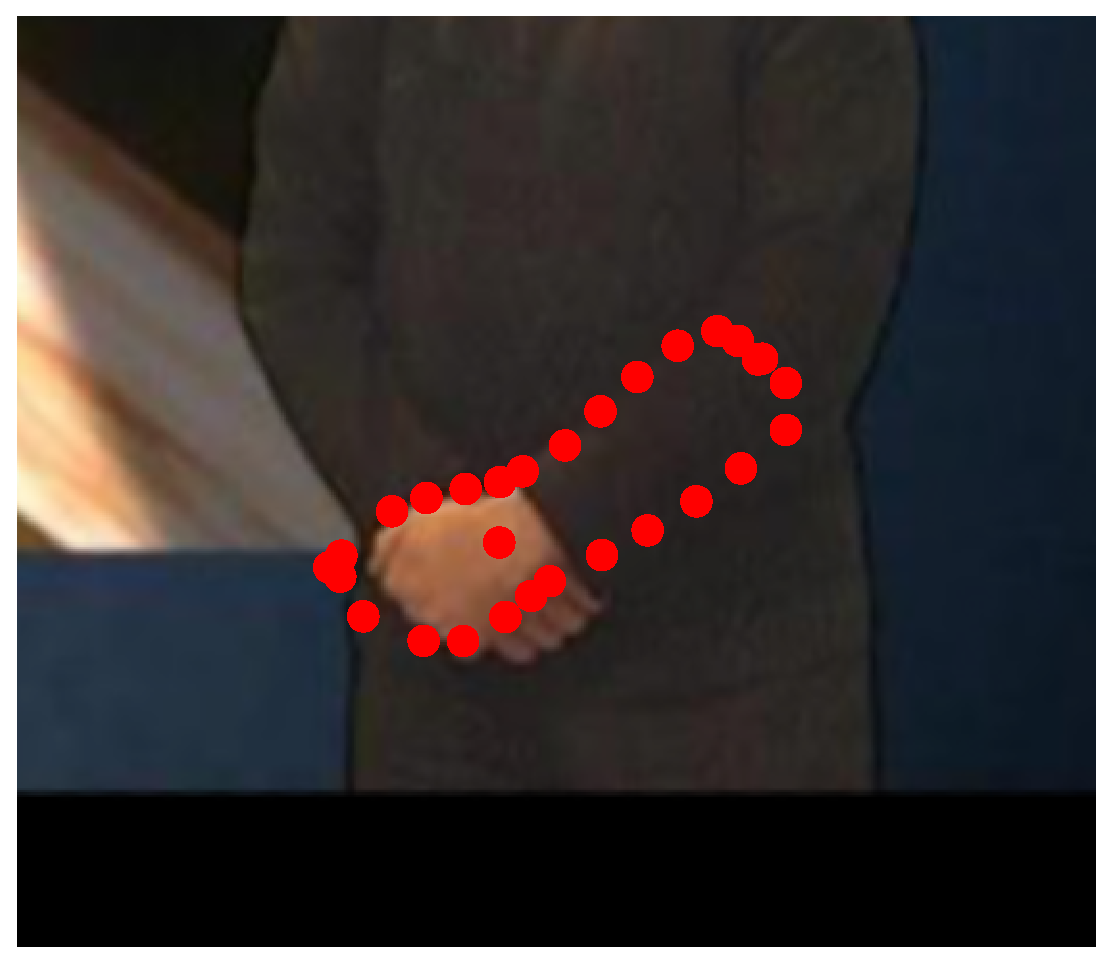
\includegraphics[height=\ofh]{Suplementory_Meterial/ExFit/0034.eps}
    \hfill
    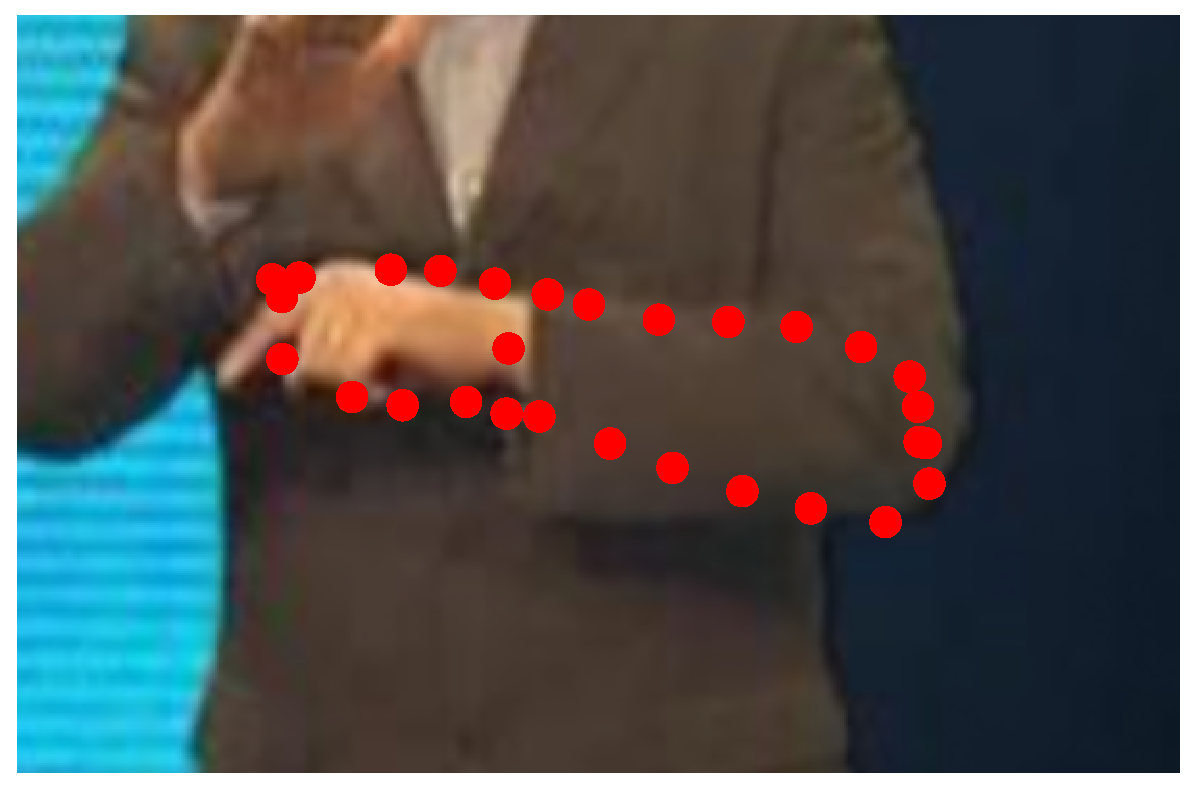
\includegraphics[height=\ofh]{Suplementory_Meterial/ExFit/0035.eps}
    \hfill
    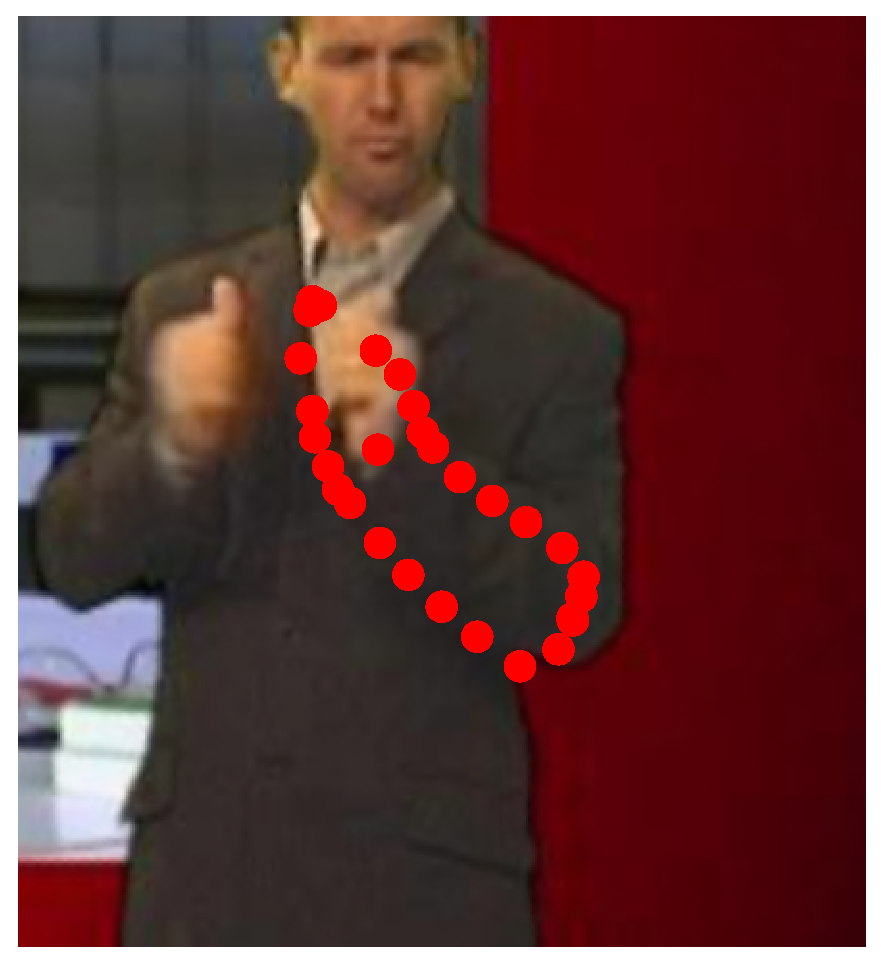
\includegraphics[height=\ofh]{Suplementory_Meterial/ExFit/0036.eps}
    \hfill
    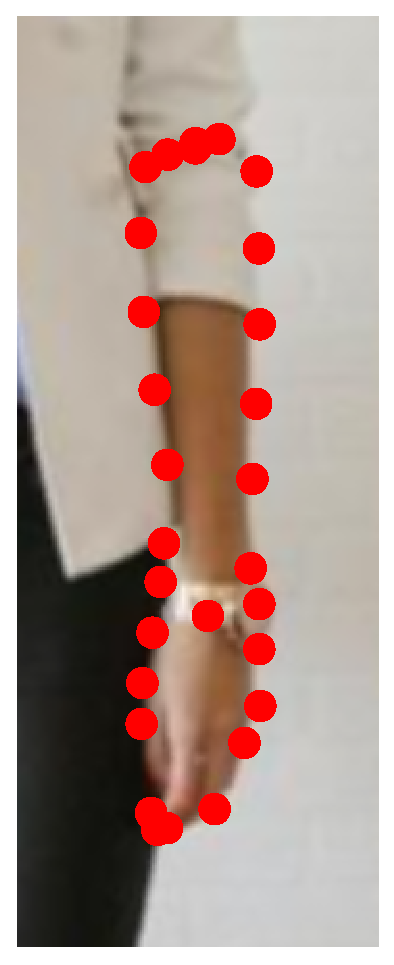
\includegraphics[height=\ofh]{Suplementory_Meterial/ExFit/0037.eps}
    \hfill
    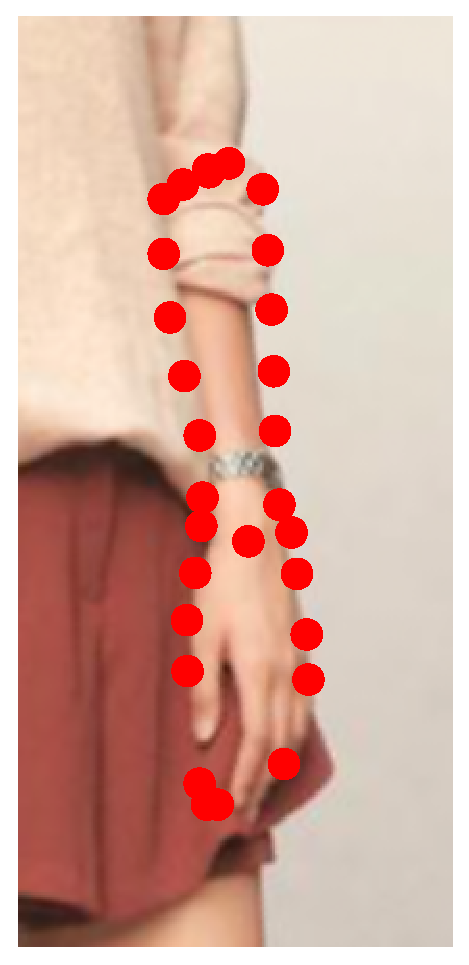
\includegraphics[height=\ofh]{Suplementory_Meterial/ExFit/0038.eps}
    \hfill
    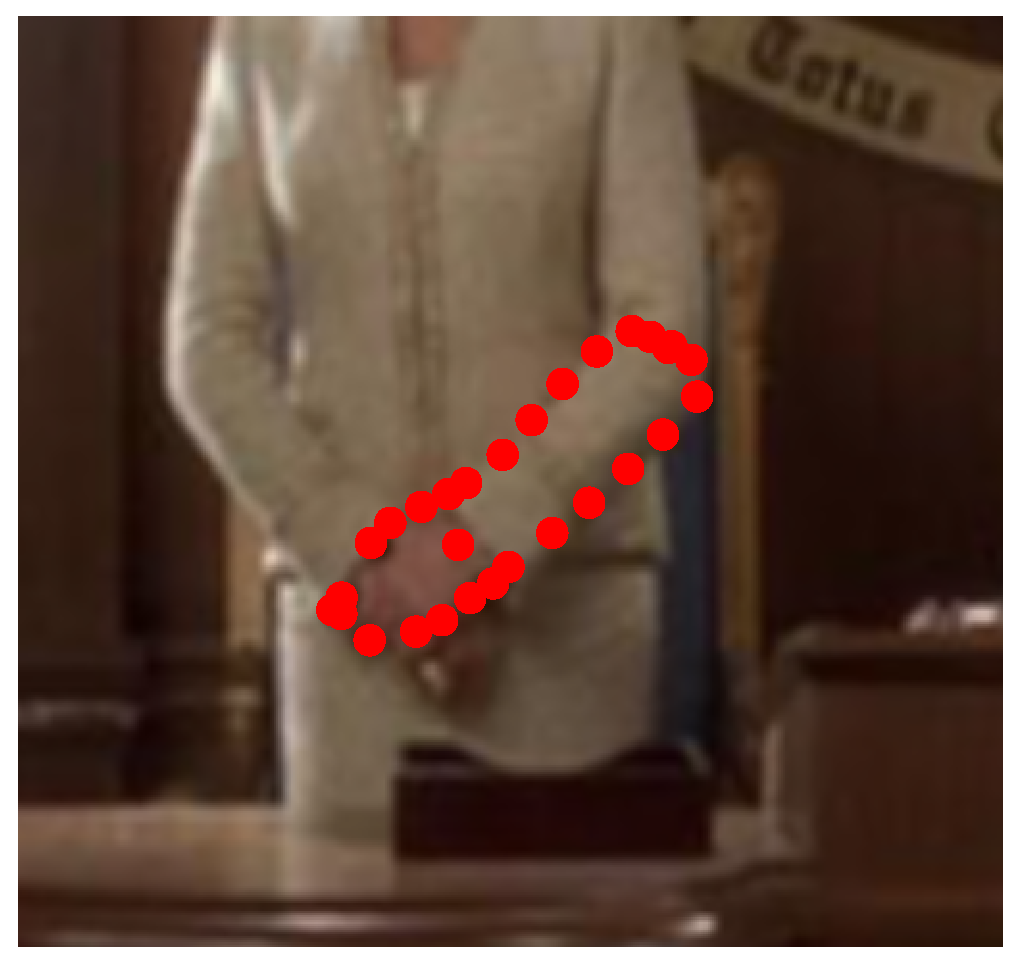
\includegraphics[height=\ofh]{Suplementory_Meterial/ExFit/0039.eps}
    \hfill
    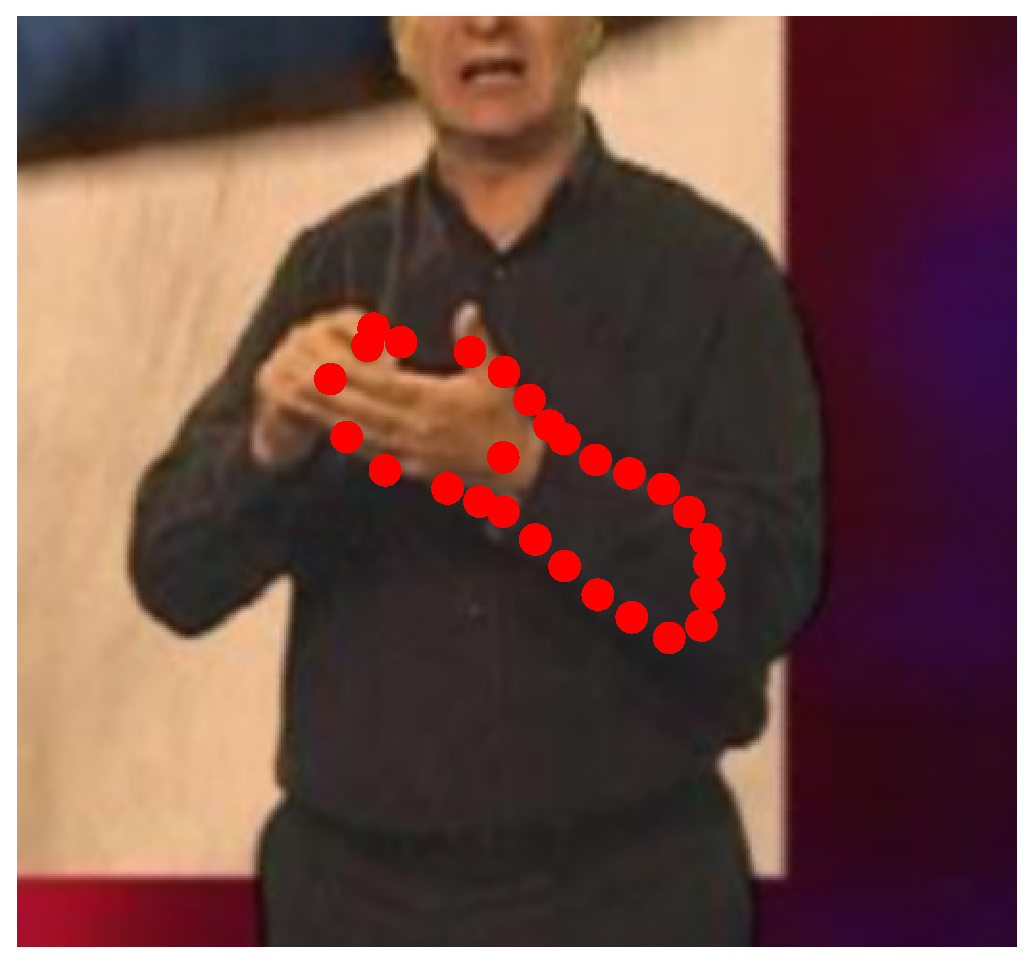
\includegraphics[height=\ofh]{Suplementory_Meterial/ExFit/0040.eps}
    \hfill
    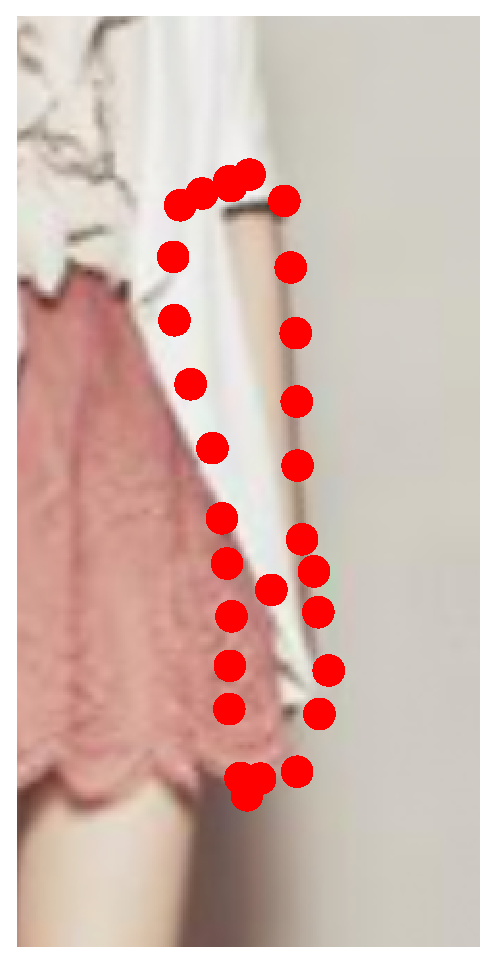
\includegraphics[height=\ofh]{Suplementory_Meterial/ExFit/0041.eps}
    \hfill
    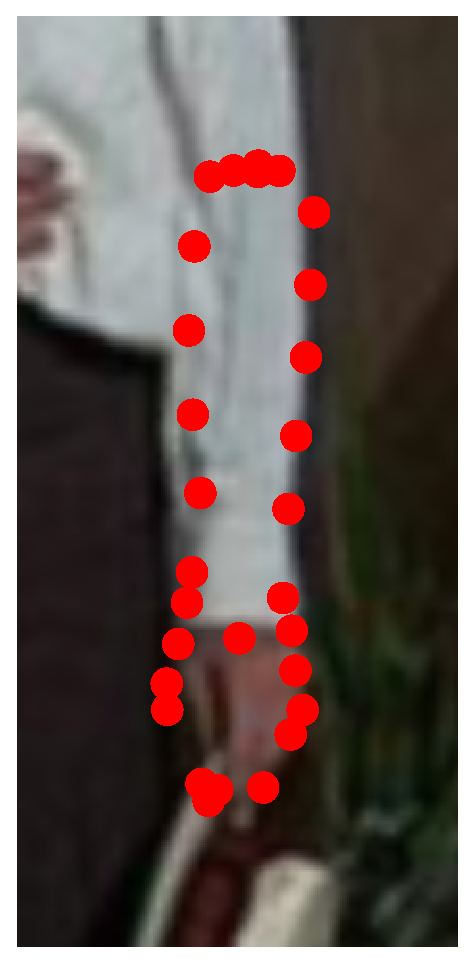
\includegraphics[height=\ofh]{Suplementory_Meterial/ExFit/0042.eps}
    \hfill
    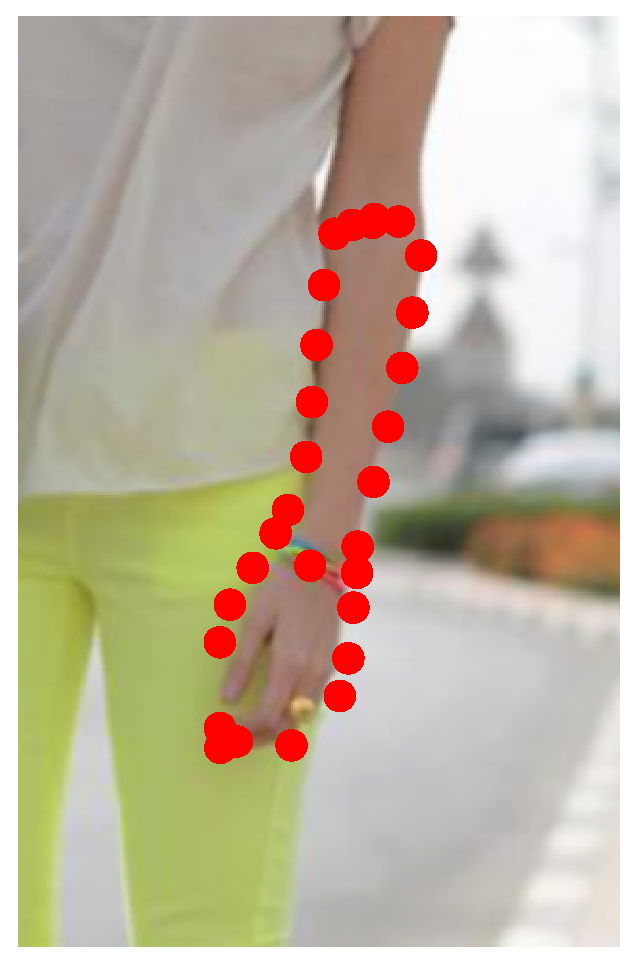
\includegraphics[height=\ofh]{Suplementory_Meterial/ExFit/0043.eps}
    \hfill
    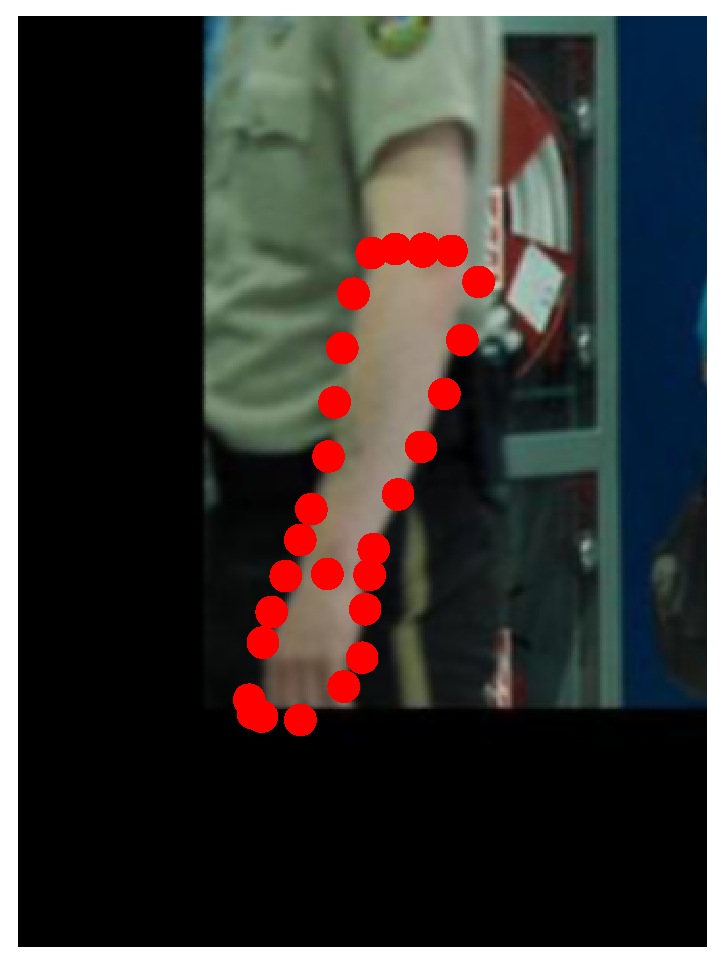
\includegraphics[height=\ofh]{Suplementory_Meterial/ExFit/0044.eps}
    \caption{Demonstration of outline fitting of patch-based AAM on arms. Images are cropped to arms only for better visualisation.}
    \label{fig:paam_fittingresults}
\end{figure*}


\subsection{Dense Fitting Visualizations}
\label{sec:daam_fittingresults}


In this section, we visualise some characteristic examples of fitting
dAAMs that were built using the proposed framework. These results are characteristic examples that come from the quantitative evaluations reported in Section 4.1 (``Non-rigid object alignment in-the-wild'') of the main paper. Figure \ref{fig:fr} shows dAAM fitting results using a grid visualisation, for both faces and ears. We observe that the proposed method successfully captures the shape deformations of these object classes and provides a detailed shape estimation for a variety of input images.


\begin{figure}[!t]
\centering
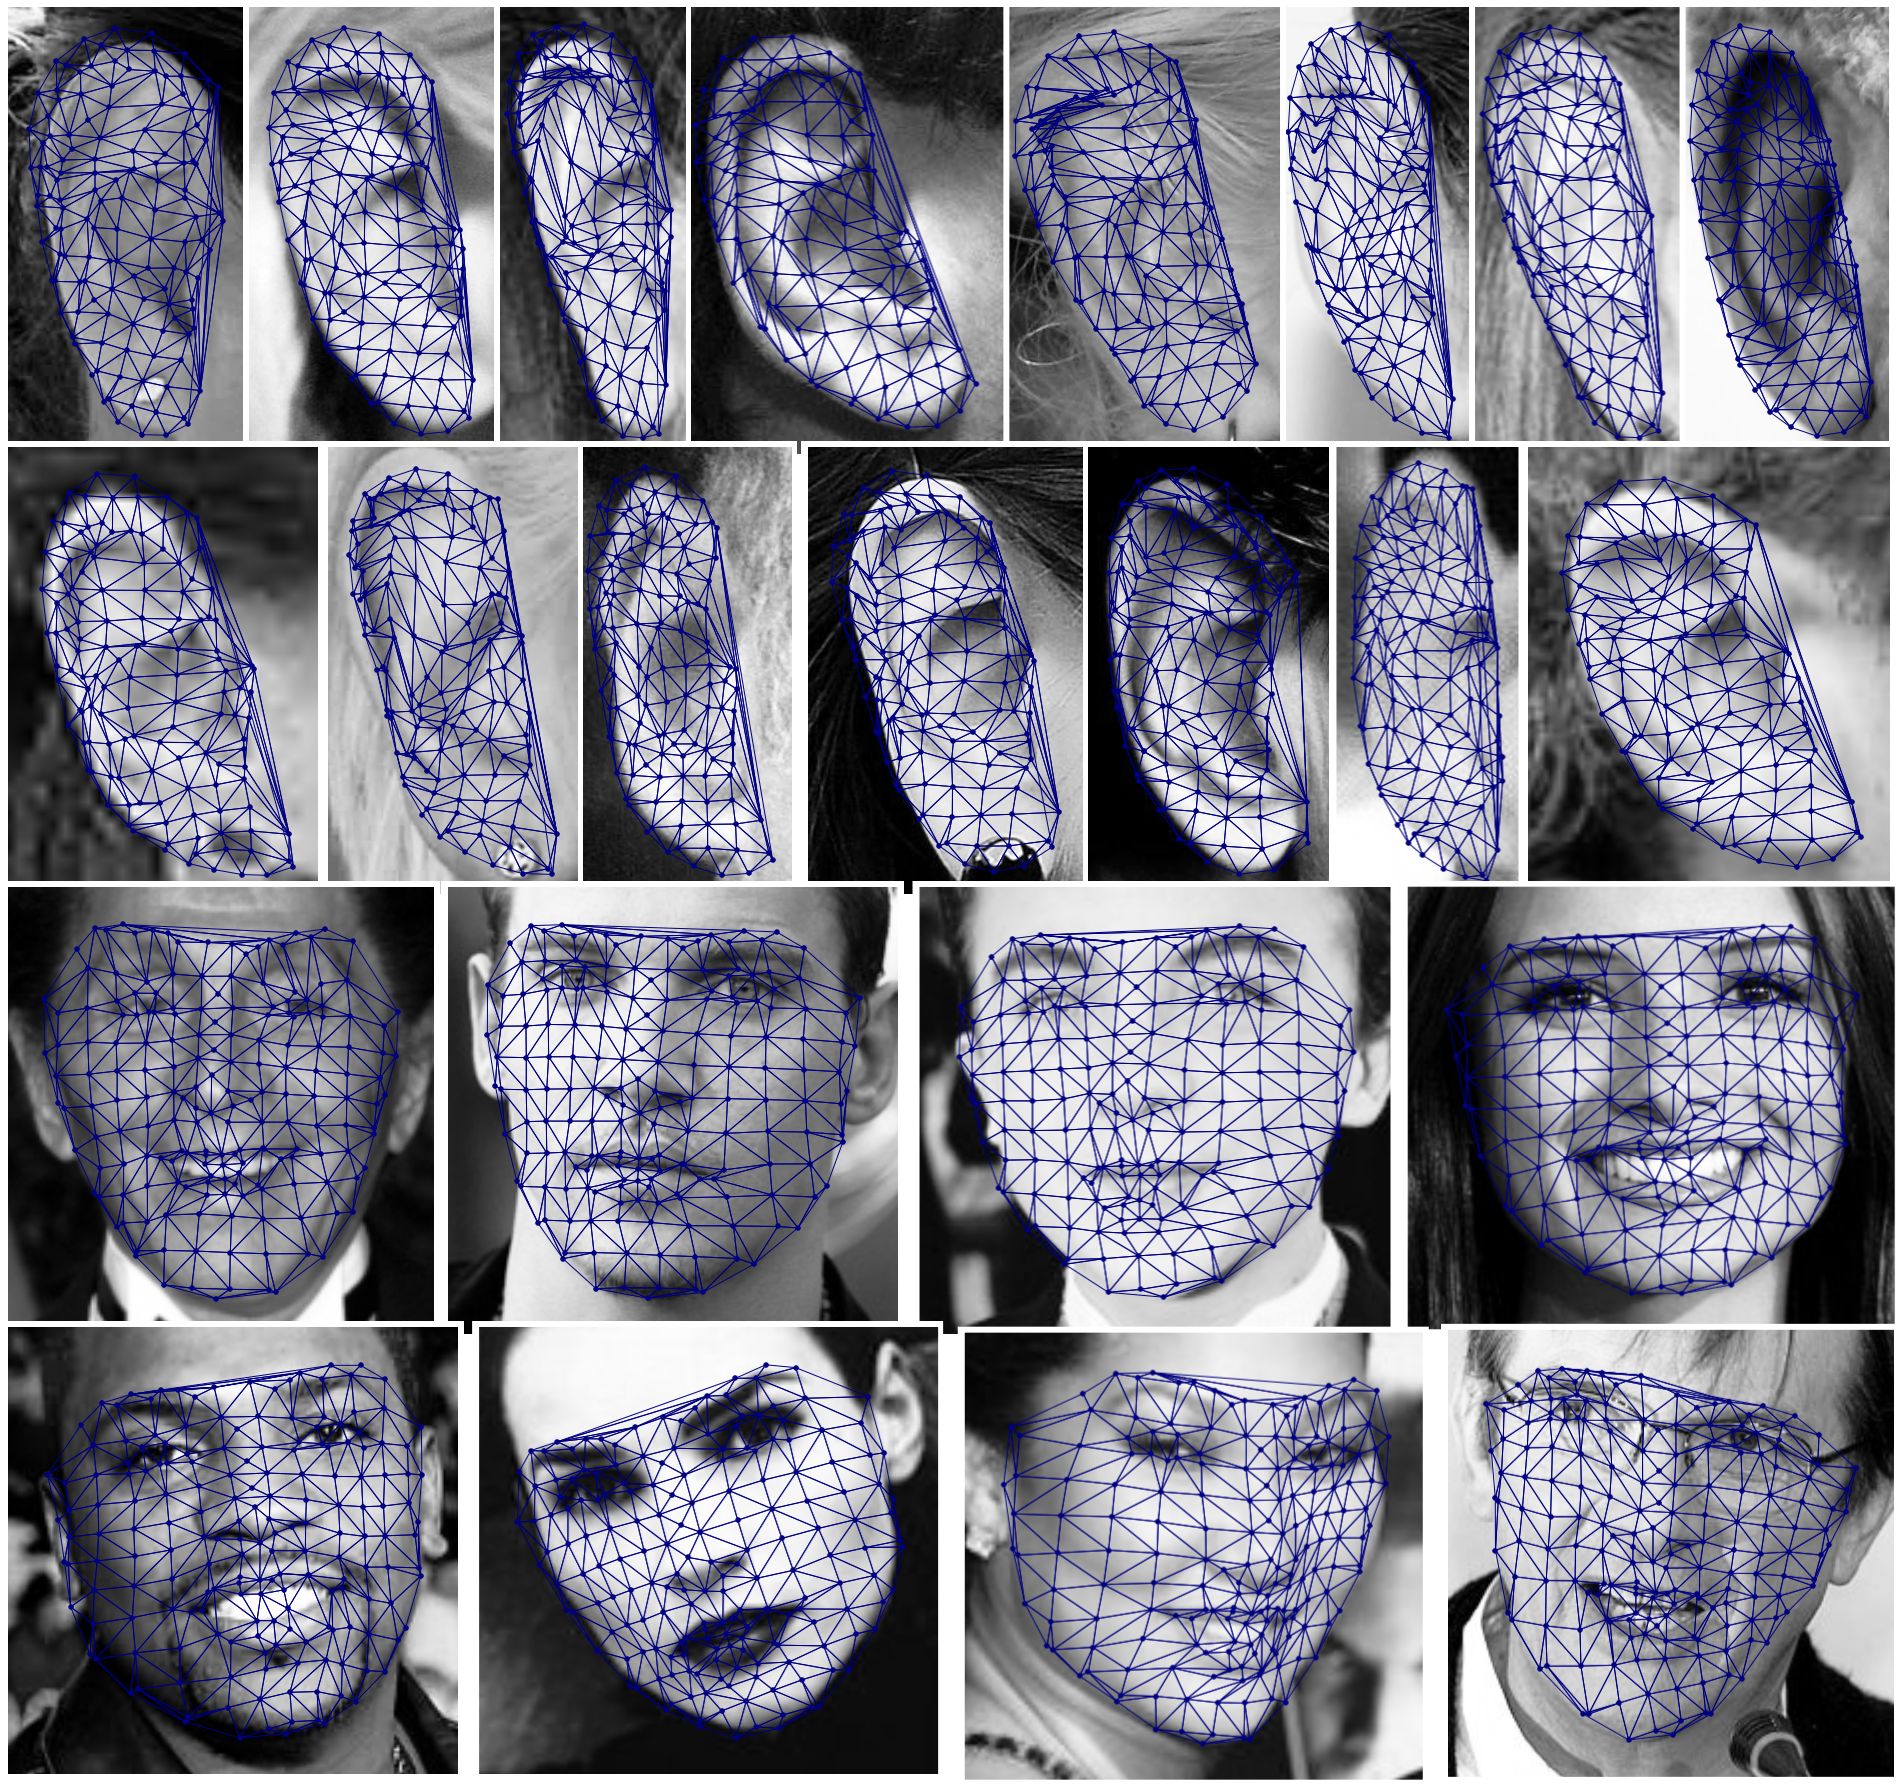
\includegraphics[width=0.5\textwidth]{Suplementory_Meterial/Fittings/fittings}
\caption{Examples of fitting
dAAMs that are constructed with the proposed pipeline. Results of dense fitting on images of
 ears (first two rows) and faces (last two rows). A grid visualisation is used.}
\label{fig:fr}
\end{figure}


\section{Patch-based Active Appearance Models}
\label{sec:paam}

In this section, we present additional visualisations and evaluations for the patch-based Active Appearance Model (PAAM) of arms that was constructed using the proposed framework.

\subsection{Subsampling of the Outline from Dense Correspondences}
\label{sec:sparsesample}

\begin{figure}[!t]
\centering
\newcommand{\ofh}{0.24\columnwidth}
    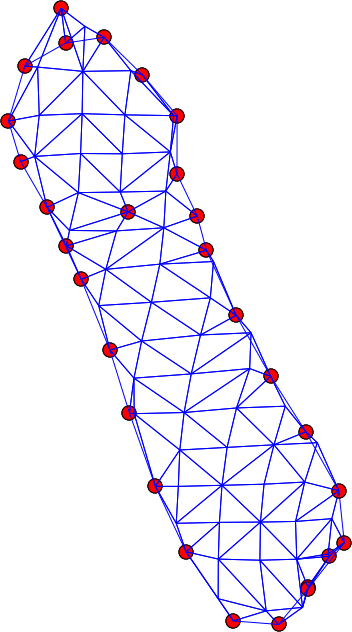
\includegraphics[height=\ofh]{Suplementory_Meterial/SparseSamples/mean.png}
    \hfill
    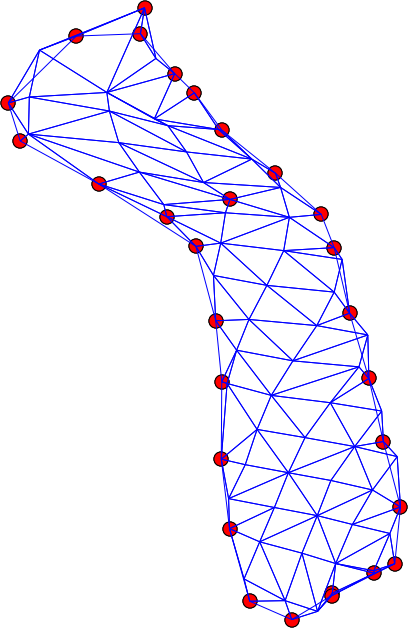
\includegraphics[height=\ofh]{Suplementory_Meterial/SparseSamples/mean-0.png}
    \hfill
    \includegraphics[height=\ofh]{Suplementory_Meterial/SparseSamples/mean-1.png}
    \hfill
    \includegraphics[height=\ofh]{Suplementory_Meterial/SparseSamples/mean-2.png}
    \hfill
    \includegraphics[height=\ofh]{Suplementory_Meterial/SparseSamples/mean-3.png}
    \hfill
    \includegraphics[height=\ofh]{Suplementory_Meterial/SparseSamples/mean-4.png}
\caption{Examples of sparse subsampling from dense shapes of arms. The dense correspondences (visualized via a deforming grid) are established using our shape flow estimation. The sparse landmarks (red dots) on the object outline are manually annotated only on the reference shape (left most image). In all other 5 example shapes, these landmarks have been automatically ``propagated'' using the established dense correspondences.}
\label{fig:sparsesample}
\end{figure}

\begin{table*}[t!]
    \centering
    \begin{tabular}{|l|c|c|c||c|c|c|}
        \hline
                            & \multicolumn{3}{c||}{Wrist} & \multicolumn{3}{c|}{Elbow}\\
        \hline
        \emph{Method}       & \emph{mean} & \emph{std} & $\leq 6pt$ & \emph{mean} & \emph{std} & $\leq 6pt$\\
        \hline\hline
        Buehler             & 12.08    & 19.94        & 44.5\%       & 12.94    & 14.65        & 34.4\%\\
        Charles14           & 11.81    & 20.89        & 54.2\%       &  8.30    & 11.00        & \textbf{55.2\%}\\
        Charles13           & 13.78    & 22.39        & 43.3\%       & 13.17    & 18.74        & 46.3\%\\
        Pfister14           & 14.69    & 17.89        & 29.7\%       & 14.60    & 10.59        & 14.0\%\\
        Ramanan             & 15.59    & 19.04        & 22.6\%       & 15.53    & 10.82        & 15.8\%\\
        Pfister15           & 7.62     & 11.04        & 54.1\%       &  8.84    & 11.44        & 54.9\%\\
        \hline\hline
        Ours                & \textbf{6.71}& \textbf{10.90}   & \textbf{63.1\%}       & \textbf{8.20}     &  \textbf{10.54}        & 52.1\%\\
        \hline
    \end{tabular}
    \caption{Fitting statistics on BBC Pose database for experiment 4.2 in main paper.}
    \label{tab:hand_benchmark}
\end{table*}

As mentioned in the main paper (Section 3 - Step 4), in order to train a PAAM, we subsample the densified training shapes to only consider points on the object's outline. Some examples of this procedure are depicted in Figure~\ref{fig:sparsesample}. We manually annotate sparse outline points only on the reference shape. Then all other training shapes are subsampled automatically exploiting the dense correspondences that are established with our shape flow estimation. We observe that the automatic subsampling seems plausible, which is attributed to the accurate estimations of dense correspondences.



\subsection{Principal Components}
\label{sec:paam_sm}



Figure~\ref{fig:paam_sm} shows the mean shape and the first 4 principal shape components of our PAAM for arms\footnote{Note that we do not visualise the appearance variation, since this is built using SIFT features and the corresponding 36-channel feature space cannot be visualised in an intuitive way.}. We observe that the shape variations captured by the model are plausible and seem to produce valid shapes of human arms.

\begin{figure}[!t]
\centering
\includegraphics[width=\columnwidth]{Suplementory_Meterial/HandSMPAAM/handsmpaam}
\caption{Principal components of our patch-based AAM for human arms.  The mean (left most column) as well as the first four principal components are visualised. $\pm 3$ times the variance of the corresponding component is used in each case.}
\label{fig:paam_sm}
\end{figure}




\subsection{Fitting Results}
\label{sec:paam_fittingresults}


Figure~\ref{fig:paam_fittingresults} demonstrates more fitting results produced by fitting patch-base AAM on arms using MPII~\cite{andriluka14cvpr}, Fashion Pose~\cite{dantone2013human}, FLIC~\cite{sapp2013modec} and BBC Pose~\cite{pfister2015flowing} databases. All fittings are initialised using the same method as mentioned in section 4.2 of the main paper.


In addition table~\ref{tab:hand_benchmark} reports statistical measures that provide additional information to section 4.2 of the main paper. Column $\leq 6pt$ reports the percentage of fittings that achieved a point-to-point normalised error less than 6 pixels (same measure used in \cite{pfister2015flowing}). This shows that we have notable improvement on estimating wrists and comparable results on estimating the elbow.







{\small
\bibliographystyle{ieee}
\bibliography{bib}
}


\end{document}






